%% Method figure (Fig. 2), full text width.  Compile with ./build.sh (pdfLaTeX, TeX Live 2026).
%% Panel (a): TikZ.  Panels (b) and (c): matplotlib PGF output (real data, see make_panels.py), typeset here.
\documentclass[10pt]{article}
\usepackage[paperwidth=6.875in,paperheight=8.82cm,margin=0pt]{geometry}
\usepackage{times}
\usepackage{amsmath,amssymb,bm,mathtools}
\usepackage[dvipsnames]{xcolor}
\usepackage{tikz}
\usetikzlibrary{arrows.meta,calc,positioning,decorations.pathreplacing,backgrounds,shapes.geometric}
% Shared method colors for all figures/diagrams (same hexes as figures/src/figstyle.py).
% Validated colorblind-safe on white (all-pairs CVD dE >= 9.4, contrast >= 3.4:1); always pair with a
% second cue (marker shape, label) so identity never relies on hue alone.
\definecolor{cOurs}{HTML}{256ABF}      % KalSea (gate + Kalman forecaster + predictor-corrector gap smoothing)
\definecolor{cKalSea}{HTML}{199E70}    % KalSea (Kalman forecasting, no smoothing)
\definecolor{cSeaCache}{HTML}{D95926}  % SeaCache (SEA gate + residual reuse)
\definecolor{cReference}{HTML}{0B0B0B} % 50-step reference
\definecolor{cInk}{HTML}{0B0B0B}
\definecolor{cInkTwo}{HTML}{52514E}
\definecolor{cMuted}{HTML}{898781}
\definecolor{cGrid}{HTML}{E1E0D9}

%% Notation for the method figure: the same definitions as paper/macros.tex (kept in sync by hand; the figure is
%% compiled stand-alone, so it cannot load macros.tex, which needs packages of the full paper build).
\newcommand{\lat}{\mathbf{x}}
\newcommand{\vel}{\mathbf{v}}
\newcommand{\hin}{\mathbf{h}^{\mathrm{in}}}
\newcommand{\hout}{\mathbf{h}^{\mathrm{out}}}
\newcommand{\res}{\mathbf{r}}
\newcommand{\resf}{\tilde{\mathbf{r}}}
\newcommand{\cond}{\mathbf{c}}
\newcommand{\blocks}{\mathcal{F}}
\DeclareMathOperator{\Emb}{Emb}
\DeclareMathOperator{\Out}{Out}
\DeclareMathOperator{\seaop}{SEA}
\DeclareMathOperator{\DCT}{DCT}
\newcommand{\modin}{\mathbf{I}}
\newcommand{\gdist}{d}
\newcommand{\kstate}{\mathbf{s}}
\newcommand{\kA}{\mathbf{A}}
\newcommand{\kP}{\mathbf{P}}
\newcommand{\kQ}{\mathbf{Q}}
\newcommand{\kPhi}{\bm{\Phi}}
\newcommand{\ds}{\Delta s}
\newcommand{\prior}[1]{#1^{-}}
\newcommand{\post}[1]{#1^{+}}
\newcommand{\smooth}[1]{#1^{\mathrm{s}}}

\pagestyle{empty}
%% double-blind / reproducible output: no file names, dates or IDs in the PDF
\pdfsuppressptexinfo=-1 \pdfinfoomitdate=1 \pdftrailerid{}
\pdfinfo{/Creator () /Producer ()}
\setlength{\parindent}{0pt}

\tikzset{
  >={Stealth[length=3.0pt,width=2.4pt]},
  every node/.style={font=\scriptsize, text=cInk},
  data/.style={->, line width=0.55pt, draw=cInk, line cap=round, line join=round},
  wire/.style={line width=0.55pt, draw=cInk, line cap=round, line join=round},
  ctrl/.style={->, line width=0.5pt, draw=cSeaCache, dash pattern=on 1.8pt off 1.1pt},
  module/.style={draw=cInk!60, line width=0.45pt, fill=black!6, rounded corners=1.2pt, minimum height=0.56cm,
                 inner sep=1.5pt, align=center},
  comp/.style={draw=#1, line width=0.6pt, fill=#1!7, rounded corners=1.6pt},
  title/.style={font=\footnotesize\bfseries, inner sep=0pt, anchor=north west},
  lbl/.style={font=\scriptsize, inner sep=1pt},
  note/.style={font=\scriptsize\itshape, text=cInkTwo, inner sep=1pt},
}

\begin{document}
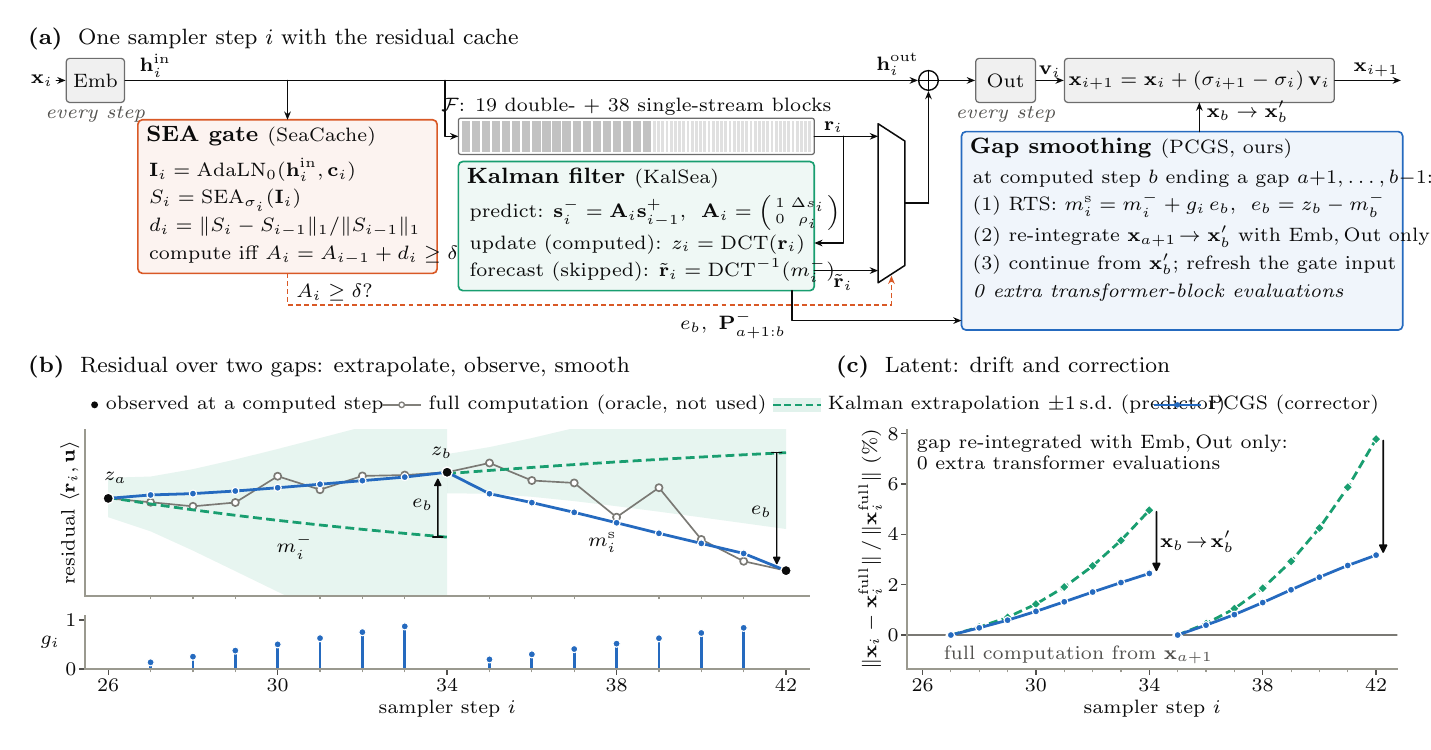
\begin{tikzpicture}[x=1cm,y=1cm]
\useasboundingbox (0,0) rectangle (17.4625,8.82);
%% ---------------------------------------------------------------- (a) top
\begin{scope}[shift={(0,5.2)}]
%% Panel (a): one sampler step with the residual cache.  TikZ commands in a local frame:
%% x in [0, 17.4625] cm (full text width), y in [-0.40, 3.62] cm.  Included by method.tex inside a shifted scope.
%% ------------------------------------------------------------------------------------------------ geometry
\def\yS{2.95}                 % spine
\def\Gx{1.40}\def\Gw{3.80}    % SEA gate box
\def\Fx{5.50}\def\Fw{4.46}    % block stack / Kalman column
\def\yF{2.24}\def\Fh{0.40}    % block stack centre, height
\def\Mx{10.80}                % residual selector (mux), left edge
\def\Px{11.44}                % adder
\def\Bx{11.86}                % PCGS box, left edge
\def\Ox{12.42}                % Out box centre
\def\Ex{14.88}                % Euler box centre
%% panel title
\node[anchor=north west, inner sep=0] at (0,3.62) {\footnotesize\textbf{(a)}\ \ One sampler step $i$ with the residual cache};

%% ------------------------------------------------------------------------------------------------ spine
\node[lbl, anchor=west] (xi) at (0,\yS) {$\lat_i$};
\node[module, minimum width=0.74cm] (emb) at (0.86,\yS) {$\Emb$};
\draw[data] (xi.east) -- (emb.west);
\node[circle, draw=cInk, line width=0.5pt, inner sep=0pt, minimum size=0.25cm, fill=white] (plus) at (\Px,\yS) {};
\draw[line width=0.5pt] (plus.north) -- (plus.south) (plus.west) -- (plus.east);
\draw[data] (emb.east) -- (plus.west);
\node[lbl, anchor=south] at (1.62,\yS) {$\hin_i$};
\node[note, anchor=north] at (0.86,\yS-0.29) {every step};

%% ------------------------------------------------------------------------------------------------ SEA gate
\draw[comp=cSeaCache] (\Gx,0.50) rectangle (\Gx+\Gw,2.45);
\node[title] at (\Gx+0.1,2.37) {SEA gate {\normalfont\scriptsize(SeaCache)}};
\node[lbl, anchor=north west, align=left] at (\Gx+0.1,2.0) {%
  $\modin_i=\mathrm{AdaLN}_0(\hin_i,\cond_i)$\\[2pt]
  $S_i=\seaop_{\sigma_i}(\modin_i)$\\[2pt]
  $d_i=\|S_i-S_{i-1}\|_1/\|S_{i-1}\|_1$\\[2pt]
  compute iff $A_i=A_{i-1}+d_i\ge\delta$};
\draw[data] (\Gx+1.9,\yS) -- (\Gx+1.9,2.45);

%% ------------------------------------------------------------------------------------------------ block stack
\pgfmathsetmacro{\unit}{\Fw/(19*2.4+38)}
\foreach \k in {0,...,18} {
  \pgfmathsetmacro{\xa}{\Fx+\k*2.4*\unit}
  \fill[black!24] (\xa+0.011,\yF-\Fh/2) rectangle (\xa+2.4*\unit-0.011,\yF+\Fh/2);
}
\foreach \k in {0,...,37} {
  \pgfmathsetmacro{\xa}{\Fx+19*2.4*\unit+\k*\unit}
  \fill[black!12] (\xa+0.009,\yF-\Fh/2) rectangle (\xa+\unit-0.009,\yF+\Fh/2);
}
\draw[cInk!60, line width=0.45pt, rounded corners=0.8pt] (\Fx-0.03,\yF-\Fh/2-0.03) rectangle (\Fx+\Fw+0.03,\yF+\Fh/2+0.03);
\node[lbl, anchor=south] at (\Fx+\Fw/2,\yF+\Fh/2+0.03) {$\blocks$: 19 double- + 38 single-stream blocks};
\draw[data] (\Fx-0.2,\yS) -- (\Fx-0.2,\yF) -- (\Fx-0.03,\yF);

%% ------------------------------------------------------------------------------------------------ Kalman filter
\draw[comp=cKalSea] (\Fx-0.03,0.28) rectangle (\Fx+\Fw+0.03,1.92);
\node[title] at (\Fx+0.07,1.84) {Kalman filter {\normalfont\scriptsize(KalSea)}};
\node[lbl, anchor=north west, align=left] at (\Fx+0.07,1.53) {%
  predict: $\prior{\kstate}_i=\kA_i\post{\kstate}_{i-1}$,\ \ $\kA_i=\begin{psmallmatrix}1&\ds_i\\0&\rho_i\end{psmallmatrix}$\\[0.5pt]
  update (computed): $z_i=\DCT(\res_i)$\\[0.5pt]
  forecast (skipped): $\resf_i=\DCT^{-1}(\prior{m}_i)$};

%% ------------------------------------------------------------------------------------------------ residual selector
\draw[wire, fill=white] (\Mx,0.38) -- (\Mx,2.40) -- (\Mx+0.34,2.18) -- (\Mx+0.34,0.60) -- cycle;
\draw[data] (\Fx+\Fw+0.03,\yF) -- node[lbl, above, pos=0.30] {$\res_i$} (\Mx,\yF);
\draw[data] (\Fx+\Fw+0.40,\yF) -- (\Fx+\Fw+0.40,0.885) -- (\Fx+\Fw+0.03,0.885);
\draw[data] (\Fx+\Fw+0.03,0.535) -- node[lbl, below, pos=0.45] {$\resf_i$} (\Mx,0.535);
\draw[wire] (\Mx+0.34,1.39) -- (\Px,1.39);
\draw[data] (\Px,1.39) -- (plus.south);
%% gate decision
\draw[ctrl] (\Gx+1.9,0.50) -- (\Gx+1.9,0.10) -- (\Mx+0.17,0.10) -- (\Mx+0.17,0.47);
\node[lbl, anchor=south west] at (\Gx+1.97,0.10) {$A_i\ge\delta$?};

%% ------------------------------------------------------------------------------------------------ output + Euler
\node[module, minimum width=0.76cm] (out) at (\Ox,\yS) {$\Out$};
\draw[data] (plus.east) -- (out.west);
\node[lbl, anchor=south east] at (\Px-0.08,\yS+0.02) {$\hout_i$};
\node[module, minimum width=3.42cm] (eul) at (\Ex,\yS) {$\lat_{i+1}=\lat_i+(\sigma_{i+1}-\sigma_i)\,\vel_i$};
\draw[data] (out.east) -- (eul.west);
\node[lbl, anchor=south] at ($(out.east)!0.5!(eul.west)$) {$\vel_i$};
\draw[data] (eul.east) -- (17.44,\yS);
\node[lbl, anchor=south east] at (17.46,\yS+0.01) {$\lat_{i+1}$};
\node[note, anchor=north] at (\Ox,\yS-0.29) {every step};

%% ------------------------------------------------------------------------------------------------ PCGS
\draw[comp=cOurs] (\Bx,-0.22) rectangle (17.4625,2.30);
\node[title] at (\Bx+0.1,2.22) {Gap smoothing {\normalfont\scriptsize(PCGS, ours)}};
\node[lbl, anchor=north west, align=left] at (\Bx+0.1,1.86) {%
  at computed step $b$ ending a gap $a{+}1,\dots,b{-}1$:\\[2pt]
  (1) RTS: $\smooth{m}_i=\prior{m}_i+g_i\,e_b$,\ \ $e_b=z_b-\prior{m}_b$\\[2pt]
  (2) re-integrate $\lat_{a+1}\!\to\lat_b'$ with $\Emb,\Out$ only\\[2pt]
  (3) continue from $\lat_b'$;\ refresh the gate input\\[2pt]
  \textit{0 extra transformer-block evaluations}};
\draw[data] (\Fx+\Fw-0.25,0.28) -- (\Fx+\Fw-0.25,-0.10) -- (\Bx,-0.10);
\node[lbl, anchor=north east] at (\Fx+\Fw-0.29,0.06) {$e_b,\ \prior{\kP}_{a+1:b}$};
\draw[data] (\Ex,2.30) -- (\Ex,\yS-0.28);
\node[lbl, anchor=west] at (\Ex+0.05,2.55) {$\lat_b\to\lat_b'$};

\end{scope}
%% ---------------------------------------------------------------- (b), (c) bottom: real trace
\node[anchor=south west, inner sep=0] at (0,0) {%% Creator: Matplotlib, PGF backend
%%
%% To include the figure in your LaTeX document, write
%%   \input{<filename>.pgf}
%%
%% Make sure the required packages are loaded in your preamble
%%   \usepackage{pgf}
%%
%% Also ensure that all the required font packages are loaded; for instance,
%% the lmodern package is sometimes necessary when using math font.
%%   \usepackage{lmodern}
%%
%% Figures using additional raster images can only be included by \input if
%% they are in the same directory as the main LaTeX file. For loading figures
%% from other directories you can use the `import` package
%%   \usepackage{import}
%%
%% and then include the figures with
%%   \import{<path to file>}{<filename>.pgf}
%%
%% Matplotlib used the following preamble
%%   \def\mathdefault#1{#1}
%%   \everymath=\expandafter{\the\everymath\displaystyle}
%%   \IfFileExists{scrextend.sty}{
%%     \usepackage[fontsize=7.000000pt]{scrextend}
%%   }{
%%     \renewcommand{\normalsize}{\fontsize{7.000000}{8.400000}\selectfont}
%%     \normalsize
%%   }
%%   \usepackage{times}
%%   \usepackage{amsmath,amssymb,bm}
%%   \input{/home/ubuntu/KalSea-dev/paper/figures/src/method/method_macros.tex}
%%   \makeatletter\@ifpackageloaded{underscore}{}{\usepackage[strings]{underscore}}\makeatother
%%
\begingroup%
\makeatletter%
\begin{pgfpicture}%
\pgfpathrectangle{\pgfpointorigin}{\pgfqpoint{3.937008in}{1.476378in}}%
\pgfusepath{use as bounding box, clip}%
\begin{pgfscope}%
\pgfsetbuttcap%
\pgfsetmiterjoin%
\definecolor{currentfill}{rgb}{1.000000,1.000000,1.000000}%
\pgfsetfillcolor{currentfill}%
\pgfsetlinewidth{0.000000pt}%
\definecolor{currentstroke}{rgb}{1.000000,1.000000,1.000000}%
\pgfsetstrokecolor{currentstroke}%
\pgfsetdash{}{0pt}%
\pgfpathmoveto{\pgfqpoint{0.000000in}{0.000000in}}%
\pgfpathlineto{\pgfqpoint{3.937008in}{0.000000in}}%
\pgfpathlineto{\pgfqpoint{3.937008in}{1.476378in}}%
\pgfpathlineto{\pgfqpoint{0.000000in}{1.476378in}}%
\pgfpathlineto{\pgfqpoint{0.000000in}{0.000000in}}%
\pgfpathclose%
\pgfusepath{fill}%
\end{pgfscope}%
\begin{pgfscope}%
\pgfsetbuttcap%
\pgfsetmiterjoin%
\definecolor{currentfill}{rgb}{1.000000,1.000000,1.000000}%
\pgfsetfillcolor{currentfill}%
\pgfsetlinewidth{0.000000pt}%
\definecolor{currentstroke}{rgb}{0.000000,0.000000,0.000000}%
\pgfsetstrokecolor{currentstroke}%
\pgfsetstrokeopacity{0.000000}%
\pgfsetdash{}{0pt}%
\pgfpathmoveto{\pgfqpoint{0.283465in}{0.627461in}}%
\pgfpathlineto{\pgfqpoint{3.905512in}{0.627461in}}%
\pgfpathlineto{\pgfqpoint{3.905512in}{1.461614in}}%
\pgfpathlineto{\pgfqpoint{0.283465in}{1.461614in}}%
\pgfpathlineto{\pgfqpoint{0.283465in}{0.627461in}}%
\pgfpathclose%
\pgfusepath{fill}%
\end{pgfscope}%
\begin{pgfscope}%
\pgfpathrectangle{\pgfqpoint{0.283465in}{0.627461in}}{\pgfqpoint{3.622047in}{0.834154in}}%
\pgfusepath{clip}%
\pgfsetbuttcap%
\pgfsetroundjoin%
\definecolor{currentfill}{rgb}{0.098039,0.619608,0.439216}%
\pgfsetfillcolor{currentfill}%
\pgfsetfillopacity{0.100000}%
\pgfsetlinewidth{0.000000pt}%
\definecolor{currentstroke}{rgb}{0.098039,0.619608,0.439216}%
\pgfsetstrokecolor{currentstroke}%
\pgfsetstrokeopacity{0.100000}%
\pgfsetdash{}{0pt}%
\pgfsys@defobject{currentmarker}{\pgfqpoint{0.399963in}{0.261367in}}{\pgfqpoint{2.094488in}{1.583211in}}{%
\pgfpathmoveto{\pgfqpoint{0.399963in}{1.219213in}}%
\pgfpathlineto{\pgfqpoint{0.399963in}{1.022053in}}%
\pgfpathlineto{\pgfqpoint{0.611779in}{0.951433in}}%
\pgfpathlineto{\pgfqpoint{0.823594in}{0.855149in}}%
\pgfpathlineto{\pgfqpoint{1.035410in}{0.752470in}}%
\pgfpathlineto{\pgfqpoint{1.247226in}{0.649410in}}%
\pgfpathlineto{\pgfqpoint{1.459041in}{0.548089in}}%
\pgfpathlineto{\pgfqpoint{1.670857in}{0.449407in}}%
\pgfpathlineto{\pgfqpoint{1.882673in}{0.353776in}}%
\pgfpathlineto{\pgfqpoint{2.094488in}{0.261367in}}%
\pgfpathlineto{\pgfqpoint{2.094488in}{1.583211in}}%
\pgfpathlineto{\pgfqpoint{2.094488in}{1.583211in}}%
\pgfpathlineto{\pgfqpoint{1.882673in}{1.528443in}}%
\pgfpathlineto{\pgfqpoint{1.670857in}{1.473139in}}%
\pgfpathlineto{\pgfqpoint{1.459041in}{1.417776in}}%
\pgfpathlineto{\pgfqpoint{1.247226in}{1.363101in}}%
\pgfpathlineto{\pgfqpoint{1.035410in}{1.310405in}}%
\pgfpathlineto{\pgfqpoint{0.823594in}{1.262270in}}%
\pgfpathlineto{\pgfqpoint{0.611779in}{1.225240in}}%
\pgfpathlineto{\pgfqpoint{0.399963in}{1.219213in}}%
\pgfpathlineto{\pgfqpoint{0.399963in}{1.219213in}}%
\pgfpathclose%
\pgfusepath{fill}%
}%
\begin{pgfscope}%
\pgfsys@transformshift{0.000000in}{0.000000in}%
\pgfsys@useobject{currentmarker}{}%
\end{pgfscope}%
\end{pgfscope}%
\begin{pgfscope}%
\pgfpathrectangle{\pgfqpoint{0.283465in}{0.627461in}}{\pgfqpoint{3.622047in}{0.834154in}}%
\pgfusepath{clip}%
\pgfsetbuttcap%
\pgfsetroundjoin%
\definecolor{currentfill}{rgb}{0.098039,0.619608,0.439216}%
\pgfsetfillcolor{currentfill}%
\pgfsetfillopacity{0.100000}%
\pgfsetlinewidth{0.000000pt}%
\definecolor{currentstroke}{rgb}{0.098039,0.619608,0.439216}%
\pgfsetstrokecolor{currentstroke}%
\pgfsetstrokeopacity{0.100000}%
\pgfsetdash{}{0pt}%
\pgfsys@defobject{currentmarker}{\pgfqpoint{2.094488in}{0.962967in}}{\pgfqpoint{3.789013in}{1.726669in}}{%
\pgfpathmoveto{\pgfqpoint{2.094488in}{1.337590in}}%
\pgfpathlineto{\pgfqpoint{2.094488in}{1.141754in}}%
\pgfpathlineto{\pgfqpoint{2.306304in}{1.139134in}}%
\pgfpathlineto{\pgfqpoint{2.518119in}{1.124150in}}%
\pgfpathlineto{\pgfqpoint{2.729935in}{1.102412in}}%
\pgfpathlineto{\pgfqpoint{2.941751in}{1.077048in}}%
\pgfpathlineto{\pgfqpoint{3.153566in}{1.049682in}}%
\pgfpathlineto{\pgfqpoint{3.365382in}{1.021220in}}%
\pgfpathlineto{\pgfqpoint{3.577198in}{0.992199in}}%
\pgfpathlineto{\pgfqpoint{3.789013in}{0.962967in}}%
\pgfpathlineto{\pgfqpoint{3.789013in}{1.726669in}}%
\pgfpathlineto{\pgfqpoint{3.789013in}{1.726669in}}%
\pgfpathlineto{\pgfqpoint{3.577198in}{1.676149in}}%
\pgfpathlineto{\pgfqpoint{3.365382in}{1.624650in}}%
\pgfpathlineto{\pgfqpoint{3.153566in}{1.572416in}}%
\pgfpathlineto{\pgfqpoint{2.941751in}{1.519875in}}%
\pgfpathlineto{\pgfqpoint{2.729935in}{1.467796in}}%
\pgfpathlineto{\pgfqpoint{2.518119in}{1.417669in}}%
\pgfpathlineto{\pgfqpoint{2.306304in}{1.372457in}}%
\pgfpathlineto{\pgfqpoint{2.094488in}{1.337590in}}%
\pgfpathlineto{\pgfqpoint{2.094488in}{1.337590in}}%
\pgfpathclose%
\pgfusepath{fill}%
}%
\begin{pgfscope}%
\pgfsys@transformshift{0.000000in}{0.000000in}%
\pgfsys@useobject{currentmarker}{}%
\end{pgfscope}%
\end{pgfscope}%
\begin{pgfscope}%
\pgfsetbuttcap%
\pgfsetroundjoin%
\definecolor{currentfill}{rgb}{0.603922,0.600000,0.560784}%
\pgfsetfillcolor{currentfill}%
\pgfsetlinewidth{0.401500pt}%
\definecolor{currentstroke}{rgb}{0.603922,0.600000,0.560784}%
\pgfsetstrokecolor{currentstroke}%
\pgfsetdash{}{0pt}%
\pgfsys@defobject{currentmarker}{\pgfqpoint{0.000000in}{-0.016667in}}{\pgfqpoint{0.000000in}{0.000000in}}{%
\pgfpathmoveto{\pgfqpoint{0.000000in}{0.000000in}}%
\pgfpathlineto{\pgfqpoint{0.000000in}{-0.016667in}}%
\pgfusepath{stroke,fill}%
}%
\begin{pgfscope}%
\pgfsys@transformshift{0.611779in}{0.627461in}%
\pgfsys@useobject{currentmarker}{}%
\end{pgfscope}%
\end{pgfscope}%
\begin{pgfscope}%
\pgfsetbuttcap%
\pgfsetroundjoin%
\definecolor{currentfill}{rgb}{0.603922,0.600000,0.560784}%
\pgfsetfillcolor{currentfill}%
\pgfsetlinewidth{0.401500pt}%
\definecolor{currentstroke}{rgb}{0.603922,0.600000,0.560784}%
\pgfsetstrokecolor{currentstroke}%
\pgfsetdash{}{0pt}%
\pgfsys@defobject{currentmarker}{\pgfqpoint{0.000000in}{-0.016667in}}{\pgfqpoint{0.000000in}{0.000000in}}{%
\pgfpathmoveto{\pgfqpoint{0.000000in}{0.000000in}}%
\pgfpathlineto{\pgfqpoint{0.000000in}{-0.016667in}}%
\pgfusepath{stroke,fill}%
}%
\begin{pgfscope}%
\pgfsys@transformshift{0.823594in}{0.627461in}%
\pgfsys@useobject{currentmarker}{}%
\end{pgfscope}%
\end{pgfscope}%
\begin{pgfscope}%
\pgfsetbuttcap%
\pgfsetroundjoin%
\definecolor{currentfill}{rgb}{0.603922,0.600000,0.560784}%
\pgfsetfillcolor{currentfill}%
\pgfsetlinewidth{0.401500pt}%
\definecolor{currentstroke}{rgb}{0.603922,0.600000,0.560784}%
\pgfsetstrokecolor{currentstroke}%
\pgfsetdash{}{0pt}%
\pgfsys@defobject{currentmarker}{\pgfqpoint{0.000000in}{-0.016667in}}{\pgfqpoint{0.000000in}{0.000000in}}{%
\pgfpathmoveto{\pgfqpoint{0.000000in}{0.000000in}}%
\pgfpathlineto{\pgfqpoint{0.000000in}{-0.016667in}}%
\pgfusepath{stroke,fill}%
}%
\begin{pgfscope}%
\pgfsys@transformshift{1.035410in}{0.627461in}%
\pgfsys@useobject{currentmarker}{}%
\end{pgfscope}%
\end{pgfscope}%
\begin{pgfscope}%
\pgfsetbuttcap%
\pgfsetroundjoin%
\definecolor{currentfill}{rgb}{0.603922,0.600000,0.560784}%
\pgfsetfillcolor{currentfill}%
\pgfsetlinewidth{0.401500pt}%
\definecolor{currentstroke}{rgb}{0.603922,0.600000,0.560784}%
\pgfsetstrokecolor{currentstroke}%
\pgfsetdash{}{0pt}%
\pgfsys@defobject{currentmarker}{\pgfqpoint{0.000000in}{-0.016667in}}{\pgfqpoint{0.000000in}{0.000000in}}{%
\pgfpathmoveto{\pgfqpoint{0.000000in}{0.000000in}}%
\pgfpathlineto{\pgfqpoint{0.000000in}{-0.016667in}}%
\pgfusepath{stroke,fill}%
}%
\begin{pgfscope}%
\pgfsys@transformshift{1.459041in}{0.627461in}%
\pgfsys@useobject{currentmarker}{}%
\end{pgfscope}%
\end{pgfscope}%
\begin{pgfscope}%
\pgfsetbuttcap%
\pgfsetroundjoin%
\definecolor{currentfill}{rgb}{0.603922,0.600000,0.560784}%
\pgfsetfillcolor{currentfill}%
\pgfsetlinewidth{0.401500pt}%
\definecolor{currentstroke}{rgb}{0.603922,0.600000,0.560784}%
\pgfsetstrokecolor{currentstroke}%
\pgfsetdash{}{0pt}%
\pgfsys@defobject{currentmarker}{\pgfqpoint{0.000000in}{-0.016667in}}{\pgfqpoint{0.000000in}{0.000000in}}{%
\pgfpathmoveto{\pgfqpoint{0.000000in}{0.000000in}}%
\pgfpathlineto{\pgfqpoint{0.000000in}{-0.016667in}}%
\pgfusepath{stroke,fill}%
}%
\begin{pgfscope}%
\pgfsys@transformshift{1.670857in}{0.627461in}%
\pgfsys@useobject{currentmarker}{}%
\end{pgfscope}%
\end{pgfscope}%
\begin{pgfscope}%
\pgfsetbuttcap%
\pgfsetroundjoin%
\definecolor{currentfill}{rgb}{0.603922,0.600000,0.560784}%
\pgfsetfillcolor{currentfill}%
\pgfsetlinewidth{0.401500pt}%
\definecolor{currentstroke}{rgb}{0.603922,0.600000,0.560784}%
\pgfsetstrokecolor{currentstroke}%
\pgfsetdash{}{0pt}%
\pgfsys@defobject{currentmarker}{\pgfqpoint{0.000000in}{-0.016667in}}{\pgfqpoint{0.000000in}{0.000000in}}{%
\pgfpathmoveto{\pgfqpoint{0.000000in}{0.000000in}}%
\pgfpathlineto{\pgfqpoint{0.000000in}{-0.016667in}}%
\pgfusepath{stroke,fill}%
}%
\begin{pgfscope}%
\pgfsys@transformshift{1.882673in}{0.627461in}%
\pgfsys@useobject{currentmarker}{}%
\end{pgfscope}%
\end{pgfscope}%
\begin{pgfscope}%
\pgfsetbuttcap%
\pgfsetroundjoin%
\definecolor{currentfill}{rgb}{0.603922,0.600000,0.560784}%
\pgfsetfillcolor{currentfill}%
\pgfsetlinewidth{0.401500pt}%
\definecolor{currentstroke}{rgb}{0.603922,0.600000,0.560784}%
\pgfsetstrokecolor{currentstroke}%
\pgfsetdash{}{0pt}%
\pgfsys@defobject{currentmarker}{\pgfqpoint{0.000000in}{-0.016667in}}{\pgfqpoint{0.000000in}{0.000000in}}{%
\pgfpathmoveto{\pgfqpoint{0.000000in}{0.000000in}}%
\pgfpathlineto{\pgfqpoint{0.000000in}{-0.016667in}}%
\pgfusepath{stroke,fill}%
}%
\begin{pgfscope}%
\pgfsys@transformshift{2.306304in}{0.627461in}%
\pgfsys@useobject{currentmarker}{}%
\end{pgfscope}%
\end{pgfscope}%
\begin{pgfscope}%
\pgfsetbuttcap%
\pgfsetroundjoin%
\definecolor{currentfill}{rgb}{0.603922,0.600000,0.560784}%
\pgfsetfillcolor{currentfill}%
\pgfsetlinewidth{0.401500pt}%
\definecolor{currentstroke}{rgb}{0.603922,0.600000,0.560784}%
\pgfsetstrokecolor{currentstroke}%
\pgfsetdash{}{0pt}%
\pgfsys@defobject{currentmarker}{\pgfqpoint{0.000000in}{-0.016667in}}{\pgfqpoint{0.000000in}{0.000000in}}{%
\pgfpathmoveto{\pgfqpoint{0.000000in}{0.000000in}}%
\pgfpathlineto{\pgfqpoint{0.000000in}{-0.016667in}}%
\pgfusepath{stroke,fill}%
}%
\begin{pgfscope}%
\pgfsys@transformshift{2.518119in}{0.627461in}%
\pgfsys@useobject{currentmarker}{}%
\end{pgfscope}%
\end{pgfscope}%
\begin{pgfscope}%
\pgfsetbuttcap%
\pgfsetroundjoin%
\definecolor{currentfill}{rgb}{0.603922,0.600000,0.560784}%
\pgfsetfillcolor{currentfill}%
\pgfsetlinewidth{0.401500pt}%
\definecolor{currentstroke}{rgb}{0.603922,0.600000,0.560784}%
\pgfsetstrokecolor{currentstroke}%
\pgfsetdash{}{0pt}%
\pgfsys@defobject{currentmarker}{\pgfqpoint{0.000000in}{-0.016667in}}{\pgfqpoint{0.000000in}{0.000000in}}{%
\pgfpathmoveto{\pgfqpoint{0.000000in}{0.000000in}}%
\pgfpathlineto{\pgfqpoint{0.000000in}{-0.016667in}}%
\pgfusepath{stroke,fill}%
}%
\begin{pgfscope}%
\pgfsys@transformshift{2.729935in}{0.627461in}%
\pgfsys@useobject{currentmarker}{}%
\end{pgfscope}%
\end{pgfscope}%
\begin{pgfscope}%
\pgfsetbuttcap%
\pgfsetroundjoin%
\definecolor{currentfill}{rgb}{0.603922,0.600000,0.560784}%
\pgfsetfillcolor{currentfill}%
\pgfsetlinewidth{0.401500pt}%
\definecolor{currentstroke}{rgb}{0.603922,0.600000,0.560784}%
\pgfsetstrokecolor{currentstroke}%
\pgfsetdash{}{0pt}%
\pgfsys@defobject{currentmarker}{\pgfqpoint{0.000000in}{-0.016667in}}{\pgfqpoint{0.000000in}{0.000000in}}{%
\pgfpathmoveto{\pgfqpoint{0.000000in}{0.000000in}}%
\pgfpathlineto{\pgfqpoint{0.000000in}{-0.016667in}}%
\pgfusepath{stroke,fill}%
}%
\begin{pgfscope}%
\pgfsys@transformshift{3.153566in}{0.627461in}%
\pgfsys@useobject{currentmarker}{}%
\end{pgfscope}%
\end{pgfscope}%
\begin{pgfscope}%
\pgfsetbuttcap%
\pgfsetroundjoin%
\definecolor{currentfill}{rgb}{0.603922,0.600000,0.560784}%
\pgfsetfillcolor{currentfill}%
\pgfsetlinewidth{0.401500pt}%
\definecolor{currentstroke}{rgb}{0.603922,0.600000,0.560784}%
\pgfsetstrokecolor{currentstroke}%
\pgfsetdash{}{0pt}%
\pgfsys@defobject{currentmarker}{\pgfqpoint{0.000000in}{-0.016667in}}{\pgfqpoint{0.000000in}{0.000000in}}{%
\pgfpathmoveto{\pgfqpoint{0.000000in}{0.000000in}}%
\pgfpathlineto{\pgfqpoint{0.000000in}{-0.016667in}}%
\pgfusepath{stroke,fill}%
}%
\begin{pgfscope}%
\pgfsys@transformshift{3.365382in}{0.627461in}%
\pgfsys@useobject{currentmarker}{}%
\end{pgfscope}%
\end{pgfscope}%
\begin{pgfscope}%
\pgfsetbuttcap%
\pgfsetroundjoin%
\definecolor{currentfill}{rgb}{0.603922,0.600000,0.560784}%
\pgfsetfillcolor{currentfill}%
\pgfsetlinewidth{0.401500pt}%
\definecolor{currentstroke}{rgb}{0.603922,0.600000,0.560784}%
\pgfsetstrokecolor{currentstroke}%
\pgfsetdash{}{0pt}%
\pgfsys@defobject{currentmarker}{\pgfqpoint{0.000000in}{-0.016667in}}{\pgfqpoint{0.000000in}{0.000000in}}{%
\pgfpathmoveto{\pgfqpoint{0.000000in}{0.000000in}}%
\pgfpathlineto{\pgfqpoint{0.000000in}{-0.016667in}}%
\pgfusepath{stroke,fill}%
}%
\begin{pgfscope}%
\pgfsys@transformshift{3.577198in}{0.627461in}%
\pgfsys@useobject{currentmarker}{}%
\end{pgfscope}%
\end{pgfscope}%
\begin{pgfscope}%
\definecolor{textcolor}{rgb}{0.043137,0.043137,0.043137}%
\pgfsetstrokecolor{textcolor}%
\pgfsetfillcolor{textcolor}%
\pgftext[x=0.255687in,y=1.044537in,,bottom,rotate=90.000000]{\color{textcolor}{\rmfamily\fontsize{7.000000}{8.400000}\selectfont\catcode`\^=\active\def^{\ifmmode\sp\else\^{}\fi}\catcode`\%=\active\def%{\%}residual $\langle\res_i,\mathbf{u}\rangle$}}%
\end{pgfscope}%
\begin{pgfscope}%
\pgfpathrectangle{\pgfqpoint{0.283465in}{0.627461in}}{\pgfqpoint{3.622047in}{0.834154in}}%
\pgfusepath{clip}%
\pgfsetroundcap%
\pgfsetroundjoin%
\pgfsetlinewidth{0.602250pt}%
\definecolor{currentstroke}{rgb}{0.478431,0.474510,0.454902}%
\pgfsetstrokecolor{currentstroke}%
\pgfsetdash{}{0pt}%
\pgfpathmoveto{\pgfqpoint{0.399963in}{1.116134in}}%
\pgfpathlineto{\pgfqpoint{0.611779in}{1.096914in}}%
\pgfpathlineto{\pgfqpoint{0.823594in}{1.076377in}}%
\pgfpathlineto{\pgfqpoint{1.035410in}{1.095501in}}%
\pgfpathlineto{\pgfqpoint{1.247226in}{1.226918in}}%
\pgfpathlineto{\pgfqpoint{1.459041in}{1.159541in}}%
\pgfpathlineto{\pgfqpoint{1.670857in}{1.228438in}}%
\pgfpathlineto{\pgfqpoint{1.882673in}{1.232660in}}%
\pgfpathlineto{\pgfqpoint{2.094488in}{1.246796in}}%
\pgfusepath{stroke}%
\end{pgfscope}%
\begin{pgfscope}%
\pgfpathrectangle{\pgfqpoint{0.283465in}{0.627461in}}{\pgfqpoint{3.622047in}{0.834154in}}%
\pgfusepath{clip}%
\pgfsetbuttcap%
\pgfsetroundjoin%
\definecolor{currentfill}{rgb}{1.000000,1.000000,1.000000}%
\pgfsetfillcolor{currentfill}%
\pgfsetlinewidth{0.602250pt}%
\definecolor{currentstroke}{rgb}{0.478431,0.474510,0.454902}%
\pgfsetstrokecolor{currentstroke}%
\pgfsetdash{}{0pt}%
\pgfsys@defobject{currentmarker}{\pgfqpoint{-0.018056in}{-0.018056in}}{\pgfqpoint{0.018056in}{0.018056in}}{%
\pgfpathmoveto{\pgfqpoint{0.000000in}{-0.018056in}}%
\pgfpathcurveto{\pgfqpoint{0.004788in}{-0.018056in}}{\pgfqpoint{0.009381in}{-0.016153in}}{\pgfqpoint{0.012767in}{-0.012767in}}%
\pgfpathcurveto{\pgfqpoint{0.016153in}{-0.009381in}}{\pgfqpoint{0.018056in}{-0.004788in}}{\pgfqpoint{0.018056in}{0.000000in}}%
\pgfpathcurveto{\pgfqpoint{0.018056in}{0.004788in}}{\pgfqpoint{0.016153in}{0.009381in}}{\pgfqpoint{0.012767in}{0.012767in}}%
\pgfpathcurveto{\pgfqpoint{0.009381in}{0.016153in}}{\pgfqpoint{0.004788in}{0.018056in}}{\pgfqpoint{0.000000in}{0.018056in}}%
\pgfpathcurveto{\pgfqpoint{-0.004788in}{0.018056in}}{\pgfqpoint{-0.009381in}{0.016153in}}{\pgfqpoint{-0.012767in}{0.012767in}}%
\pgfpathcurveto{\pgfqpoint{-0.016153in}{0.009381in}}{\pgfqpoint{-0.018056in}{0.004788in}}{\pgfqpoint{-0.018056in}{0.000000in}}%
\pgfpathcurveto{\pgfqpoint{-0.018056in}{-0.004788in}}{\pgfqpoint{-0.016153in}{-0.009381in}}{\pgfqpoint{-0.012767in}{-0.012767in}}%
\pgfpathcurveto{\pgfqpoint{-0.009381in}{-0.016153in}}{\pgfqpoint{-0.004788in}{-0.018056in}}{\pgfqpoint{0.000000in}{-0.018056in}}%
\pgfpathlineto{\pgfqpoint{0.000000in}{-0.018056in}}%
\pgfpathclose%
\pgfusepath{stroke,fill}%
}%
\begin{pgfscope}%
\pgfsys@transformshift{0.611779in}{1.096914in}%
\pgfsys@useobject{currentmarker}{}%
\end{pgfscope}%
\begin{pgfscope}%
\pgfsys@transformshift{0.823594in}{1.076377in}%
\pgfsys@useobject{currentmarker}{}%
\end{pgfscope}%
\begin{pgfscope}%
\pgfsys@transformshift{1.035410in}{1.095501in}%
\pgfsys@useobject{currentmarker}{}%
\end{pgfscope}%
\begin{pgfscope}%
\pgfsys@transformshift{1.247226in}{1.226918in}%
\pgfsys@useobject{currentmarker}{}%
\end{pgfscope}%
\begin{pgfscope}%
\pgfsys@transformshift{1.459041in}{1.159541in}%
\pgfsys@useobject{currentmarker}{}%
\end{pgfscope}%
\begin{pgfscope}%
\pgfsys@transformshift{1.670857in}{1.228438in}%
\pgfsys@useobject{currentmarker}{}%
\end{pgfscope}%
\begin{pgfscope}%
\pgfsys@transformshift{1.882673in}{1.232660in}%
\pgfsys@useobject{currentmarker}{}%
\end{pgfscope}%
\end{pgfscope}%
\begin{pgfscope}%
\pgfpathrectangle{\pgfqpoint{0.283465in}{0.627461in}}{\pgfqpoint{3.622047in}{0.834154in}}%
\pgfusepath{clip}%
\pgfsetroundcap%
\pgfsetroundjoin%
\pgfsetlinewidth{0.602250pt}%
\definecolor{currentstroke}{rgb}{0.478431,0.474510,0.454902}%
\pgfsetstrokecolor{currentstroke}%
\pgfsetdash{}{0pt}%
\pgfpathmoveto{\pgfqpoint{2.094488in}{1.246796in}}%
\pgfpathlineto{\pgfqpoint{2.306304in}{1.293123in}}%
\pgfpathlineto{\pgfqpoint{2.518119in}{1.205427in}}%
\pgfpathlineto{\pgfqpoint{2.729935in}{1.193391in}}%
\pgfpathlineto{\pgfqpoint{2.941751in}{1.022192in}}%
\pgfpathlineto{\pgfqpoint{3.153566in}{1.169622in}}%
\pgfpathlineto{\pgfqpoint{3.365382in}{0.910690in}}%
\pgfpathlineto{\pgfqpoint{3.577198in}{0.801698in}}%
\pgfpathlineto{\pgfqpoint{3.789013in}{0.754901in}}%
\pgfusepath{stroke}%
\end{pgfscope}%
\begin{pgfscope}%
\pgfpathrectangle{\pgfqpoint{0.283465in}{0.627461in}}{\pgfqpoint{3.622047in}{0.834154in}}%
\pgfusepath{clip}%
\pgfsetbuttcap%
\pgfsetroundjoin%
\definecolor{currentfill}{rgb}{1.000000,1.000000,1.000000}%
\pgfsetfillcolor{currentfill}%
\pgfsetlinewidth{0.602250pt}%
\definecolor{currentstroke}{rgb}{0.478431,0.474510,0.454902}%
\pgfsetstrokecolor{currentstroke}%
\pgfsetdash{}{0pt}%
\pgfsys@defobject{currentmarker}{\pgfqpoint{-0.018056in}{-0.018056in}}{\pgfqpoint{0.018056in}{0.018056in}}{%
\pgfpathmoveto{\pgfqpoint{0.000000in}{-0.018056in}}%
\pgfpathcurveto{\pgfqpoint{0.004788in}{-0.018056in}}{\pgfqpoint{0.009381in}{-0.016153in}}{\pgfqpoint{0.012767in}{-0.012767in}}%
\pgfpathcurveto{\pgfqpoint{0.016153in}{-0.009381in}}{\pgfqpoint{0.018056in}{-0.004788in}}{\pgfqpoint{0.018056in}{0.000000in}}%
\pgfpathcurveto{\pgfqpoint{0.018056in}{0.004788in}}{\pgfqpoint{0.016153in}{0.009381in}}{\pgfqpoint{0.012767in}{0.012767in}}%
\pgfpathcurveto{\pgfqpoint{0.009381in}{0.016153in}}{\pgfqpoint{0.004788in}{0.018056in}}{\pgfqpoint{0.000000in}{0.018056in}}%
\pgfpathcurveto{\pgfqpoint{-0.004788in}{0.018056in}}{\pgfqpoint{-0.009381in}{0.016153in}}{\pgfqpoint{-0.012767in}{0.012767in}}%
\pgfpathcurveto{\pgfqpoint{-0.016153in}{0.009381in}}{\pgfqpoint{-0.018056in}{0.004788in}}{\pgfqpoint{-0.018056in}{0.000000in}}%
\pgfpathcurveto{\pgfqpoint{-0.018056in}{-0.004788in}}{\pgfqpoint{-0.016153in}{-0.009381in}}{\pgfqpoint{-0.012767in}{-0.012767in}}%
\pgfpathcurveto{\pgfqpoint{-0.009381in}{-0.016153in}}{\pgfqpoint{-0.004788in}{-0.018056in}}{\pgfqpoint{0.000000in}{-0.018056in}}%
\pgfpathlineto{\pgfqpoint{0.000000in}{-0.018056in}}%
\pgfpathclose%
\pgfusepath{stroke,fill}%
}%
\begin{pgfscope}%
\pgfsys@transformshift{2.306304in}{1.293123in}%
\pgfsys@useobject{currentmarker}{}%
\end{pgfscope}%
\begin{pgfscope}%
\pgfsys@transformshift{2.518119in}{1.205427in}%
\pgfsys@useobject{currentmarker}{}%
\end{pgfscope}%
\begin{pgfscope}%
\pgfsys@transformshift{2.729935in}{1.193391in}%
\pgfsys@useobject{currentmarker}{}%
\end{pgfscope}%
\begin{pgfscope}%
\pgfsys@transformshift{2.941751in}{1.022192in}%
\pgfsys@useobject{currentmarker}{}%
\end{pgfscope}%
\begin{pgfscope}%
\pgfsys@transformshift{3.153566in}{1.169622in}%
\pgfsys@useobject{currentmarker}{}%
\end{pgfscope}%
\begin{pgfscope}%
\pgfsys@transformshift{3.365382in}{0.910690in}%
\pgfsys@useobject{currentmarker}{}%
\end{pgfscope}%
\begin{pgfscope}%
\pgfsys@transformshift{3.577198in}{0.801698in}%
\pgfsys@useobject{currentmarker}{}%
\end{pgfscope}%
\end{pgfscope}%
\begin{pgfscope}%
\pgfsetrectcap%
\pgfsetmiterjoin%
\pgfsetlinewidth{0.501875pt}%
\definecolor{currentstroke}{rgb}{0.603922,0.600000,0.560784}%
\pgfsetstrokecolor{currentstroke}%
\pgfsetdash{}{0pt}%
\pgfpathmoveto{\pgfqpoint{0.283465in}{0.627461in}}%
\pgfpathlineto{\pgfqpoint{0.283465in}{1.461614in}}%
\pgfusepath{stroke}%
\end{pgfscope}%
\begin{pgfscope}%
\pgfsetrectcap%
\pgfsetmiterjoin%
\pgfsetlinewidth{0.501875pt}%
\definecolor{currentstroke}{rgb}{0.603922,0.600000,0.560784}%
\pgfsetstrokecolor{currentstroke}%
\pgfsetdash{}{0pt}%
\pgfpathmoveto{\pgfqpoint{0.283465in}{0.627461in}}%
\pgfpathlineto{\pgfqpoint{3.905512in}{0.627461in}}%
\pgfusepath{stroke}%
\end{pgfscope}%
\begin{pgfscope}%
\pgfpathrectangle{\pgfqpoint{0.283465in}{0.627461in}}{\pgfqpoint{3.622047in}{0.834154in}}%
\pgfusepath{clip}%
\pgfsetbuttcap%
\pgfsetroundjoin%
\pgfsetlinewidth{1.003750pt}%
\definecolor{currentstroke}{rgb}{0.098039,0.619608,0.439216}%
\pgfsetstrokecolor{currentstroke}%
\pgfsetdash{{3.200000pt}{1.600000pt}}{0.000000pt}%
\pgfpathmoveto{\pgfqpoint{0.399963in}{1.120633in}}%
\pgfpathlineto{\pgfqpoint{0.611779in}{1.088337in}}%
\pgfpathlineto{\pgfqpoint{0.823594in}{1.058710in}}%
\pgfpathlineto{\pgfqpoint{1.035410in}{1.031437in}}%
\pgfpathlineto{\pgfqpoint{1.247226in}{1.006255in}}%
\pgfpathlineto{\pgfqpoint{1.459041in}{0.982932in}}%
\pgfpathlineto{\pgfqpoint{1.670857in}{0.961273in}}%
\pgfpathlineto{\pgfqpoint{1.882673in}{0.941109in}}%
\pgfpathlineto{\pgfqpoint{2.094488in}{0.922289in}}%
\pgfusepath{stroke}%
\end{pgfscope}%
\begin{pgfscope}%
\pgfpathrectangle{\pgfqpoint{0.283465in}{0.627461in}}{\pgfqpoint{3.622047in}{0.834154in}}%
\pgfusepath{clip}%
\pgfsetbuttcap%
\pgfsetroundjoin%
\pgfsetlinewidth{1.003750pt}%
\definecolor{currentstroke}{rgb}{0.098039,0.619608,0.439216}%
\pgfsetstrokecolor{currentstroke}%
\pgfsetdash{{3.200000pt}{1.600000pt}}{0.000000pt}%
\pgfpathmoveto{\pgfqpoint{2.094488in}{1.239672in}}%
\pgfpathlineto{\pgfqpoint{2.306304in}{1.255796in}}%
\pgfpathlineto{\pgfqpoint{2.518119in}{1.270910in}}%
\pgfpathlineto{\pgfqpoint{2.729935in}{1.285104in}}%
\pgfpathlineto{\pgfqpoint{2.941751in}{1.298461in}}%
\pgfpathlineto{\pgfqpoint{3.153566in}{1.311049in}}%
\pgfpathlineto{\pgfqpoint{3.365382in}{1.322935in}}%
\pgfpathlineto{\pgfqpoint{3.577198in}{1.334174in}}%
\pgfpathlineto{\pgfqpoint{3.789013in}{1.344818in}}%
\pgfusepath{stroke}%
\end{pgfscope}%
\begin{pgfscope}%
\definecolor{textcolor}{rgb}{0.043137,0.043137,0.043137}%
\pgfsetstrokecolor{textcolor}%
\pgfsetfillcolor{textcolor}%
\pgftext[x=0.379130in,y=1.192522in,left,bottom]{\color{textcolor}{\rmfamily\fontsize{7.000000}{8.400000}\selectfont\catcode`\^=\active\def^{\ifmmode\sp\else\^{}\fi}\catcode`\%=\active\def%{\%}$z_a$}}%
\end{pgfscope}%
\begin{pgfscope}%
\definecolor{textcolor}{rgb}{0.043137,0.043137,0.043137}%
\pgfsetstrokecolor{textcolor}%
\pgfsetfillcolor{textcolor}%
\pgftext[x=2.066710in,y=1.316240in,,bottom]{\color{textcolor}{\rmfamily\fontsize{7.000000}{8.400000}\selectfont\catcode`\^=\active\def^{\ifmmode\sp\else\^{}\fi}\catcode`\%=\active\def%{\%}$z_b$}}%
\end{pgfscope}%
\begin{pgfscope}%
\definecolor{textcolor}{rgb}{0.043137,0.043137,0.043137}%
\pgfsetstrokecolor{textcolor}%
\pgfsetfillcolor{textcolor}%
\pgftext[x=1.331952in,y=0.934426in,,top]{\color{textcolor}{\rmfamily\fontsize{7.000000}{8.400000}\selectfont\catcode`\^=\active\def^{\ifmmode\sp\else\^{}\fi}\catcode`\%=\active\def%{\%}$\prior{m}_i$}}%
\end{pgfscope}%
\begin{pgfscope}%
\definecolor{textcolor}{rgb}{0.043137,0.043137,0.043137}%
\pgfsetstrokecolor{textcolor}%
\pgfsetfillcolor{textcolor}%
\pgftext[x=2.870913in,y=0.945569in,,top]{\color{textcolor}{\rmfamily\fontsize{7.000000}{8.400000}\selectfont\catcode`\^=\active\def^{\ifmmode\sp\else\^{}\fi}\catcode`\%=\active\def%{\%}$\smooth{m}_i$}}%
\end{pgfscope}%
\begin{pgfscope}%
\pgfpathrectangle{\pgfqpoint{0.283465in}{0.627461in}}{\pgfqpoint{3.622047in}{0.834154in}}%
\pgfusepath{clip}%
\pgfsetroundcap%
\pgfsetroundjoin%
\pgfsetlinewidth{1.003750pt}%
\definecolor{currentstroke}{rgb}{0.145098,0.415686,0.749020}%
\pgfsetstrokecolor{currentstroke}%
\pgfsetdash{}{0pt}%
\pgfpathmoveto{\pgfqpoint{0.399963in}{1.116134in}}%
\pgfpathlineto{\pgfqpoint{0.611779in}{1.133265in}}%
\pgfpathlineto{\pgfqpoint{0.823594in}{1.140022in}}%
\pgfpathlineto{\pgfqpoint{1.035410in}{1.152954in}}%
\pgfpathlineto{\pgfqpoint{1.247226in}{1.169290in}}%
\pgfpathlineto{\pgfqpoint{1.459041in}{1.186834in}}%
\pgfpathlineto{\pgfqpoint{1.670857in}{1.204776in}}%
\pgfpathlineto{\pgfqpoint{1.882673in}{1.222605in}}%
\pgfpathlineto{\pgfqpoint{2.094488in}{1.246796in}}%
\pgfusepath{stroke}%
\end{pgfscope}%
\begin{pgfscope}%
\pgfpathrectangle{\pgfqpoint{0.283465in}{0.627461in}}{\pgfqpoint{3.622047in}{0.834154in}}%
\pgfusepath{clip}%
\pgfsetbuttcap%
\pgfsetroundjoin%
\definecolor{currentfill}{rgb}{0.145098,0.415686,0.749020}%
\pgfsetfillcolor{currentfill}%
\pgfsetlinewidth{0.401500pt}%
\definecolor{currentstroke}{rgb}{1.000000,1.000000,1.000000}%
\pgfsetstrokecolor{currentstroke}%
\pgfsetdash{}{0pt}%
\pgfsys@defobject{currentmarker}{\pgfqpoint{-0.018056in}{-0.018056in}}{\pgfqpoint{0.018056in}{0.018056in}}{%
\pgfpathmoveto{\pgfqpoint{0.000000in}{-0.018056in}}%
\pgfpathcurveto{\pgfqpoint{0.004788in}{-0.018056in}}{\pgfqpoint{0.009381in}{-0.016153in}}{\pgfqpoint{0.012767in}{-0.012767in}}%
\pgfpathcurveto{\pgfqpoint{0.016153in}{-0.009381in}}{\pgfqpoint{0.018056in}{-0.004788in}}{\pgfqpoint{0.018056in}{0.000000in}}%
\pgfpathcurveto{\pgfqpoint{0.018056in}{0.004788in}}{\pgfqpoint{0.016153in}{0.009381in}}{\pgfqpoint{0.012767in}{0.012767in}}%
\pgfpathcurveto{\pgfqpoint{0.009381in}{0.016153in}}{\pgfqpoint{0.004788in}{0.018056in}}{\pgfqpoint{0.000000in}{0.018056in}}%
\pgfpathcurveto{\pgfqpoint{-0.004788in}{0.018056in}}{\pgfqpoint{-0.009381in}{0.016153in}}{\pgfqpoint{-0.012767in}{0.012767in}}%
\pgfpathcurveto{\pgfqpoint{-0.016153in}{0.009381in}}{\pgfqpoint{-0.018056in}{0.004788in}}{\pgfqpoint{-0.018056in}{0.000000in}}%
\pgfpathcurveto{\pgfqpoint{-0.018056in}{-0.004788in}}{\pgfqpoint{-0.016153in}{-0.009381in}}{\pgfqpoint{-0.012767in}{-0.012767in}}%
\pgfpathcurveto{\pgfqpoint{-0.009381in}{-0.016153in}}{\pgfqpoint{-0.004788in}{-0.018056in}}{\pgfqpoint{0.000000in}{-0.018056in}}%
\pgfpathlineto{\pgfqpoint{0.000000in}{-0.018056in}}%
\pgfpathclose%
\pgfusepath{stroke,fill}%
}%
\begin{pgfscope}%
\pgfsys@transformshift{0.611779in}{1.133265in}%
\pgfsys@useobject{currentmarker}{}%
\end{pgfscope}%
\begin{pgfscope}%
\pgfsys@transformshift{0.823594in}{1.140022in}%
\pgfsys@useobject{currentmarker}{}%
\end{pgfscope}%
\begin{pgfscope}%
\pgfsys@transformshift{1.035410in}{1.152954in}%
\pgfsys@useobject{currentmarker}{}%
\end{pgfscope}%
\begin{pgfscope}%
\pgfsys@transformshift{1.247226in}{1.169290in}%
\pgfsys@useobject{currentmarker}{}%
\end{pgfscope}%
\begin{pgfscope}%
\pgfsys@transformshift{1.459041in}{1.186834in}%
\pgfsys@useobject{currentmarker}{}%
\end{pgfscope}%
\begin{pgfscope}%
\pgfsys@transformshift{1.670857in}{1.204776in}%
\pgfsys@useobject{currentmarker}{}%
\end{pgfscope}%
\begin{pgfscope}%
\pgfsys@transformshift{1.882673in}{1.222605in}%
\pgfsys@useobject{currentmarker}{}%
\end{pgfscope}%
\end{pgfscope}%
\begin{pgfscope}%
\pgfpathrectangle{\pgfqpoint{0.283465in}{0.627461in}}{\pgfqpoint{3.622047in}{0.834154in}}%
\pgfusepath{clip}%
\pgfsetroundcap%
\pgfsetroundjoin%
\pgfsetlinewidth{1.003750pt}%
\definecolor{currentstroke}{rgb}{0.145098,0.415686,0.749020}%
\pgfsetstrokecolor{currentstroke}%
\pgfsetdash{}{0pt}%
\pgfpathmoveto{\pgfqpoint{2.094488in}{1.246796in}}%
\pgfpathlineto{\pgfqpoint{2.306304in}{1.139378in}}%
\pgfpathlineto{\pgfqpoint{2.518119in}{1.095031in}}%
\pgfpathlineto{\pgfqpoint{2.729935in}{1.046280in}}%
\pgfpathlineto{\pgfqpoint{2.941751in}{0.994169in}}%
\pgfpathlineto{\pgfqpoint{3.153566in}{0.941349in}}%
\pgfpathlineto{\pgfqpoint{3.365382in}{0.891023in}}%
\pgfpathlineto{\pgfqpoint{3.577198in}{0.840818in}}%
\pgfpathlineto{\pgfqpoint{3.789013in}{0.754901in}}%
\pgfusepath{stroke}%
\end{pgfscope}%
\begin{pgfscope}%
\pgfpathrectangle{\pgfqpoint{0.283465in}{0.627461in}}{\pgfqpoint{3.622047in}{0.834154in}}%
\pgfusepath{clip}%
\pgfsetbuttcap%
\pgfsetroundjoin%
\definecolor{currentfill}{rgb}{0.145098,0.415686,0.749020}%
\pgfsetfillcolor{currentfill}%
\pgfsetlinewidth{0.401500pt}%
\definecolor{currentstroke}{rgb}{1.000000,1.000000,1.000000}%
\pgfsetstrokecolor{currentstroke}%
\pgfsetdash{}{0pt}%
\pgfsys@defobject{currentmarker}{\pgfqpoint{-0.018056in}{-0.018056in}}{\pgfqpoint{0.018056in}{0.018056in}}{%
\pgfpathmoveto{\pgfqpoint{0.000000in}{-0.018056in}}%
\pgfpathcurveto{\pgfqpoint{0.004788in}{-0.018056in}}{\pgfqpoint{0.009381in}{-0.016153in}}{\pgfqpoint{0.012767in}{-0.012767in}}%
\pgfpathcurveto{\pgfqpoint{0.016153in}{-0.009381in}}{\pgfqpoint{0.018056in}{-0.004788in}}{\pgfqpoint{0.018056in}{0.000000in}}%
\pgfpathcurveto{\pgfqpoint{0.018056in}{0.004788in}}{\pgfqpoint{0.016153in}{0.009381in}}{\pgfqpoint{0.012767in}{0.012767in}}%
\pgfpathcurveto{\pgfqpoint{0.009381in}{0.016153in}}{\pgfqpoint{0.004788in}{0.018056in}}{\pgfqpoint{0.000000in}{0.018056in}}%
\pgfpathcurveto{\pgfqpoint{-0.004788in}{0.018056in}}{\pgfqpoint{-0.009381in}{0.016153in}}{\pgfqpoint{-0.012767in}{0.012767in}}%
\pgfpathcurveto{\pgfqpoint{-0.016153in}{0.009381in}}{\pgfqpoint{-0.018056in}{0.004788in}}{\pgfqpoint{-0.018056in}{0.000000in}}%
\pgfpathcurveto{\pgfqpoint{-0.018056in}{-0.004788in}}{\pgfqpoint{-0.016153in}{-0.009381in}}{\pgfqpoint{-0.012767in}{-0.012767in}}%
\pgfpathcurveto{\pgfqpoint{-0.009381in}{-0.016153in}}{\pgfqpoint{-0.004788in}{-0.018056in}}{\pgfqpoint{0.000000in}{-0.018056in}}%
\pgfpathlineto{\pgfqpoint{0.000000in}{-0.018056in}}%
\pgfpathclose%
\pgfusepath{stroke,fill}%
}%
\begin{pgfscope}%
\pgfsys@transformshift{2.306304in}{1.139378in}%
\pgfsys@useobject{currentmarker}{}%
\end{pgfscope}%
\begin{pgfscope}%
\pgfsys@transformshift{2.518119in}{1.095031in}%
\pgfsys@useobject{currentmarker}{}%
\end{pgfscope}%
\begin{pgfscope}%
\pgfsys@transformshift{2.729935in}{1.046280in}%
\pgfsys@useobject{currentmarker}{}%
\end{pgfscope}%
\begin{pgfscope}%
\pgfsys@transformshift{2.941751in}{0.994169in}%
\pgfsys@useobject{currentmarker}{}%
\end{pgfscope}%
\begin{pgfscope}%
\pgfsys@transformshift{3.153566in}{0.941349in}%
\pgfsys@useobject{currentmarker}{}%
\end{pgfscope}%
\begin{pgfscope}%
\pgfsys@transformshift{3.365382in}{0.891023in}%
\pgfsys@useobject{currentmarker}{}%
\end{pgfscope}%
\begin{pgfscope}%
\pgfsys@transformshift{3.577198in}{0.840818in}%
\pgfsys@useobject{currentmarker}{}%
\end{pgfscope}%
\end{pgfscope}%
\begin{pgfscope}%
\pgfpathrectangle{\pgfqpoint{0.283465in}{0.627461in}}{\pgfqpoint{3.622047in}{0.834154in}}%
\pgfusepath{clip}%
\pgfsetroundcap%
\pgfsetroundjoin%
\pgfsetlinewidth{0.501875pt}%
\definecolor{currentstroke}{rgb}{0.043137,0.043137,0.043137}%
\pgfsetstrokecolor{currentstroke}%
\pgfsetdash{}{0pt}%
\pgfpathmoveto{\pgfqpoint{2.047889in}{0.922289in}}%
\pgfpathquadraticcurveto{\pgfqpoint{2.047889in}{1.070658in}}{\pgfqpoint{2.047889in}{1.211263in}}%
\pgfusepath{stroke}%
\end{pgfscope}%
\begin{pgfscope}%
\pgfpathrectangle{\pgfqpoint{0.283465in}{0.627461in}}{\pgfqpoint{3.622047in}{0.834154in}}%
\pgfusepath{clip}%
\pgfsetroundcap%
\pgfsetroundjoin%
\definecolor{currentfill}{rgb}{0.043137,0.043137,0.043137}%
\pgfsetfillcolor{currentfill}%
\pgfsetlinewidth{0.501875pt}%
\definecolor{currentstroke}{rgb}{0.043137,0.043137,0.043137}%
\pgfsetstrokecolor{currentstroke}%
\pgfsetdash{}{0pt}%
\pgfpathmoveto{\pgfqpoint{2.032611in}{1.180707in}}%
\pgfpathlineto{\pgfqpoint{2.047889in}{1.211263in}}%
\pgfpathlineto{\pgfqpoint{2.063167in}{1.180707in}}%
\pgfpathlineto{\pgfqpoint{2.032611in}{1.180707in}}%
\pgfpathclose%
\pgfusepath{stroke,fill}%
\end{pgfscope}%
\begin{pgfscope}%
\pgfpathrectangle{\pgfqpoint{0.283465in}{0.627461in}}{\pgfqpoint{3.622047in}{0.834154in}}%
\pgfusepath{clip}%
\pgfsetroundcap%
\pgfsetroundjoin%
\pgfsetlinewidth{0.501875pt}%
\definecolor{currentstroke}{rgb}{0.043137,0.043137,0.043137}%
\pgfsetstrokecolor{currentstroke}%
\pgfsetdash{}{0pt}%
\pgfpathmoveto{\pgfqpoint{2.022471in}{0.922289in}}%
\pgfpathlineto{\pgfqpoint{2.073307in}{0.922289in}}%
\pgfusepath{stroke}%
\end{pgfscope}%
\begin{pgfscope}%
\definecolor{textcolor}{rgb}{0.043137,0.043137,0.043137}%
\pgfsetstrokecolor{textcolor}%
\pgfsetfillcolor{textcolor}%
\pgftext[x=2.022471in,y=1.084542in,right,]{\color{textcolor}{\rmfamily\fontsize{7.000000}{8.400000}\selectfont\catcode`\^=\active\def^{\ifmmode\sp\else\^{}\fi}\catcode`\%=\active\def%{\%}$e_b$}}%
\end{pgfscope}%
\begin{pgfscope}%
\pgfpathrectangle{\pgfqpoint{0.283465in}{0.627461in}}{\pgfqpoint{3.622047in}{0.834154in}}%
\pgfusepath{clip}%
\pgfsetroundcap%
\pgfsetroundjoin%
\pgfsetlinewidth{0.501875pt}%
\definecolor{currentstroke}{rgb}{0.043137,0.043137,0.043137}%
\pgfsetstrokecolor{currentstroke}%
\pgfsetdash{}{0pt}%
\pgfpathmoveto{\pgfqpoint{3.742414in}{1.344818in}}%
\pgfpathquadraticcurveto{\pgfqpoint{3.742414in}{1.063740in}}{\pgfqpoint{3.742414in}{0.790425in}}%
\pgfusepath{stroke}%
\end{pgfscope}%
\begin{pgfscope}%
\pgfpathrectangle{\pgfqpoint{0.283465in}{0.627461in}}{\pgfqpoint{3.622047in}{0.834154in}}%
\pgfusepath{clip}%
\pgfsetroundcap%
\pgfsetroundjoin%
\definecolor{currentfill}{rgb}{0.043137,0.043137,0.043137}%
\pgfsetfillcolor{currentfill}%
\pgfsetlinewidth{0.501875pt}%
\definecolor{currentstroke}{rgb}{0.043137,0.043137,0.043137}%
\pgfsetstrokecolor{currentstroke}%
\pgfsetdash{}{0pt}%
\pgfpathmoveto{\pgfqpoint{3.757692in}{0.820981in}}%
\pgfpathlineto{\pgfqpoint{3.742414in}{0.790425in}}%
\pgfpathlineto{\pgfqpoint{3.727136in}{0.820981in}}%
\pgfpathlineto{\pgfqpoint{3.757692in}{0.820981in}}%
\pgfpathclose%
\pgfusepath{stroke,fill}%
\end{pgfscope}%
\begin{pgfscope}%
\pgfpathrectangle{\pgfqpoint{0.283465in}{0.627461in}}{\pgfqpoint{3.622047in}{0.834154in}}%
\pgfusepath{clip}%
\pgfsetroundcap%
\pgfsetroundjoin%
\pgfsetlinewidth{0.501875pt}%
\definecolor{currentstroke}{rgb}{0.043137,0.043137,0.043137}%
\pgfsetstrokecolor{currentstroke}%
\pgfsetdash{}{0pt}%
\pgfpathmoveto{\pgfqpoint{3.716996in}{1.344818in}}%
\pgfpathlineto{\pgfqpoint{3.767832in}{1.344818in}}%
\pgfusepath{stroke}%
\end{pgfscope}%
\begin{pgfscope}%
\definecolor{textcolor}{rgb}{0.043137,0.043137,0.043137}%
\pgfsetstrokecolor{textcolor}%
\pgfsetfillcolor{textcolor}%
\pgftext[x=3.716996in,y=1.049859in,right,]{\color{textcolor}{\rmfamily\fontsize{7.000000}{8.400000}\selectfont\catcode`\^=\active\def^{\ifmmode\sp\else\^{}\fi}\catcode`\%=\active\def%{\%}$e_b$}}%
\end{pgfscope}%
\begin{pgfscope}%
\pgfpathrectangle{\pgfqpoint{0.283465in}{0.627461in}}{\pgfqpoint{3.622047in}{0.834154in}}%
\pgfusepath{clip}%
\pgfsetbuttcap%
\pgfsetroundjoin%
\definecolor{currentfill}{rgb}{0.043137,0.043137,0.043137}%
\pgfsetfillcolor{currentfill}%
\pgfsetlinewidth{0.501875pt}%
\definecolor{currentstroke}{rgb}{1.000000,1.000000,1.000000}%
\pgfsetstrokecolor{currentstroke}%
\pgfsetdash{}{0pt}%
\pgfsys@defobject{currentmarker}{\pgfqpoint{-0.026389in}{-0.026389in}}{\pgfqpoint{0.026389in}{0.026389in}}{%
\pgfpathmoveto{\pgfqpoint{0.000000in}{-0.026389in}}%
\pgfpathcurveto{\pgfqpoint{0.006998in}{-0.026389in}}{\pgfqpoint{0.013711in}{-0.023608in}}{\pgfqpoint{0.018660in}{-0.018660in}}%
\pgfpathcurveto{\pgfqpoint{0.023608in}{-0.013711in}}{\pgfqpoint{0.026389in}{-0.006998in}}{\pgfqpoint{0.026389in}{0.000000in}}%
\pgfpathcurveto{\pgfqpoint{0.026389in}{0.006998in}}{\pgfqpoint{0.023608in}{0.013711in}}{\pgfqpoint{0.018660in}{0.018660in}}%
\pgfpathcurveto{\pgfqpoint{0.013711in}{0.023608in}}{\pgfqpoint{0.006998in}{0.026389in}}{\pgfqpoint{0.000000in}{0.026389in}}%
\pgfpathcurveto{\pgfqpoint{-0.006998in}{0.026389in}}{\pgfqpoint{-0.013711in}{0.023608in}}{\pgfqpoint{-0.018660in}{0.018660in}}%
\pgfpathcurveto{\pgfqpoint{-0.023608in}{0.013711in}}{\pgfqpoint{-0.026389in}{0.006998in}}{\pgfqpoint{-0.026389in}{0.000000in}}%
\pgfpathcurveto{\pgfqpoint{-0.026389in}{-0.006998in}}{\pgfqpoint{-0.023608in}{-0.013711in}}{\pgfqpoint{-0.018660in}{-0.018660in}}%
\pgfpathcurveto{\pgfqpoint{-0.013711in}{-0.023608in}}{\pgfqpoint{-0.006998in}{-0.026389in}}{\pgfqpoint{0.000000in}{-0.026389in}}%
\pgfpathlineto{\pgfqpoint{0.000000in}{-0.026389in}}%
\pgfpathclose%
\pgfusepath{stroke,fill}%
}%
\begin{pgfscope}%
\pgfsys@transformshift{0.399963in}{1.116134in}%
\pgfsys@useobject{currentmarker}{}%
\end{pgfscope}%
\begin{pgfscope}%
\pgfsys@transformshift{2.094488in}{1.246796in}%
\pgfsys@useobject{currentmarker}{}%
\end{pgfscope}%
\begin{pgfscope}%
\pgfsys@transformshift{3.789013in}{0.754901in}%
\pgfsys@useobject{currentmarker}{}%
\end{pgfscope}%
\end{pgfscope}%
\begin{pgfscope}%
\pgfsetbuttcap%
\pgfsetmiterjoin%
\definecolor{currentfill}{rgb}{1.000000,1.000000,1.000000}%
\pgfsetfillcolor{currentfill}%
\pgfsetlinewidth{0.000000pt}%
\definecolor{currentstroke}{rgb}{0.000000,0.000000,0.000000}%
\pgfsetstrokecolor{currentstroke}%
\pgfsetstrokeopacity{0.000000}%
\pgfsetdash{}{0pt}%
\pgfpathmoveto{\pgfqpoint{0.283465in}{0.262795in}}%
\pgfpathlineto{\pgfqpoint{3.905512in}{0.262795in}}%
\pgfpathlineto{\pgfqpoint{3.905512in}{0.528543in}}%
\pgfpathlineto{\pgfqpoint{0.283465in}{0.528543in}}%
\pgfpathlineto{\pgfqpoint{0.283465in}{0.262795in}}%
\pgfpathclose%
\pgfusepath{fill}%
\end{pgfscope}%
\begin{pgfscope}%
\pgfsetbuttcap%
\pgfsetroundjoin%
\definecolor{currentfill}{rgb}{0.321569,0.317647,0.305882}%
\pgfsetfillcolor{currentfill}%
\pgfsetlinewidth{0.501875pt}%
\definecolor{currentstroke}{rgb}{0.321569,0.317647,0.305882}%
\pgfsetstrokecolor{currentstroke}%
\pgfsetdash{}{0pt}%
\pgfsys@defobject{currentmarker}{\pgfqpoint{0.000000in}{-0.027778in}}{\pgfqpoint{0.000000in}{0.000000in}}{%
\pgfpathmoveto{\pgfqpoint{0.000000in}{0.000000in}}%
\pgfpathlineto{\pgfqpoint{0.000000in}{-0.027778in}}%
\pgfusepath{stroke,fill}%
}%
\begin{pgfscope}%
\pgfsys@transformshift{0.399963in}{0.262795in}%
\pgfsys@useobject{currentmarker}{}%
\end{pgfscope}%
\end{pgfscope}%
\begin{pgfscope}%
\definecolor{textcolor}{rgb}{0.043137,0.043137,0.043137}%
\pgfsetstrokecolor{textcolor}%
\pgfsetfillcolor{textcolor}%
\pgftext[x=0.399963in,y=0.214184in,,top]{\color{textcolor}{\rmfamily\fontsize{7.000000}{8.400000}\selectfont\catcode`\^=\active\def^{\ifmmode\sp\else\^{}\fi}\catcode`\%=\active\def%{\%}26}}%
\end{pgfscope}%
\begin{pgfscope}%
\pgfsetbuttcap%
\pgfsetroundjoin%
\definecolor{currentfill}{rgb}{0.321569,0.317647,0.305882}%
\pgfsetfillcolor{currentfill}%
\pgfsetlinewidth{0.501875pt}%
\definecolor{currentstroke}{rgb}{0.321569,0.317647,0.305882}%
\pgfsetstrokecolor{currentstroke}%
\pgfsetdash{}{0pt}%
\pgfsys@defobject{currentmarker}{\pgfqpoint{0.000000in}{-0.027778in}}{\pgfqpoint{0.000000in}{0.000000in}}{%
\pgfpathmoveto{\pgfqpoint{0.000000in}{0.000000in}}%
\pgfpathlineto{\pgfqpoint{0.000000in}{-0.027778in}}%
\pgfusepath{stroke,fill}%
}%
\begin{pgfscope}%
\pgfsys@transformshift{1.247226in}{0.262795in}%
\pgfsys@useobject{currentmarker}{}%
\end{pgfscope}%
\end{pgfscope}%
\begin{pgfscope}%
\definecolor{textcolor}{rgb}{0.043137,0.043137,0.043137}%
\pgfsetstrokecolor{textcolor}%
\pgfsetfillcolor{textcolor}%
\pgftext[x=1.247226in,y=0.214184in,,top]{\color{textcolor}{\rmfamily\fontsize{7.000000}{8.400000}\selectfont\catcode`\^=\active\def^{\ifmmode\sp\else\^{}\fi}\catcode`\%=\active\def%{\%}30}}%
\end{pgfscope}%
\begin{pgfscope}%
\pgfsetbuttcap%
\pgfsetroundjoin%
\definecolor{currentfill}{rgb}{0.321569,0.317647,0.305882}%
\pgfsetfillcolor{currentfill}%
\pgfsetlinewidth{0.501875pt}%
\definecolor{currentstroke}{rgb}{0.321569,0.317647,0.305882}%
\pgfsetstrokecolor{currentstroke}%
\pgfsetdash{}{0pt}%
\pgfsys@defobject{currentmarker}{\pgfqpoint{0.000000in}{-0.027778in}}{\pgfqpoint{0.000000in}{0.000000in}}{%
\pgfpathmoveto{\pgfqpoint{0.000000in}{0.000000in}}%
\pgfpathlineto{\pgfqpoint{0.000000in}{-0.027778in}}%
\pgfusepath{stroke,fill}%
}%
\begin{pgfscope}%
\pgfsys@transformshift{2.094488in}{0.262795in}%
\pgfsys@useobject{currentmarker}{}%
\end{pgfscope}%
\end{pgfscope}%
\begin{pgfscope}%
\definecolor{textcolor}{rgb}{0.043137,0.043137,0.043137}%
\pgfsetstrokecolor{textcolor}%
\pgfsetfillcolor{textcolor}%
\pgftext[x=2.094488in,y=0.214184in,,top]{\color{textcolor}{\rmfamily\fontsize{7.000000}{8.400000}\selectfont\catcode`\^=\active\def^{\ifmmode\sp\else\^{}\fi}\catcode`\%=\active\def%{\%}34}}%
\end{pgfscope}%
\begin{pgfscope}%
\pgfsetbuttcap%
\pgfsetroundjoin%
\definecolor{currentfill}{rgb}{0.321569,0.317647,0.305882}%
\pgfsetfillcolor{currentfill}%
\pgfsetlinewidth{0.501875pt}%
\definecolor{currentstroke}{rgb}{0.321569,0.317647,0.305882}%
\pgfsetstrokecolor{currentstroke}%
\pgfsetdash{}{0pt}%
\pgfsys@defobject{currentmarker}{\pgfqpoint{0.000000in}{-0.027778in}}{\pgfqpoint{0.000000in}{0.000000in}}{%
\pgfpathmoveto{\pgfqpoint{0.000000in}{0.000000in}}%
\pgfpathlineto{\pgfqpoint{0.000000in}{-0.027778in}}%
\pgfusepath{stroke,fill}%
}%
\begin{pgfscope}%
\pgfsys@transformshift{2.941751in}{0.262795in}%
\pgfsys@useobject{currentmarker}{}%
\end{pgfscope}%
\end{pgfscope}%
\begin{pgfscope}%
\definecolor{textcolor}{rgb}{0.043137,0.043137,0.043137}%
\pgfsetstrokecolor{textcolor}%
\pgfsetfillcolor{textcolor}%
\pgftext[x=2.941751in,y=0.214184in,,top]{\color{textcolor}{\rmfamily\fontsize{7.000000}{8.400000}\selectfont\catcode`\^=\active\def^{\ifmmode\sp\else\^{}\fi}\catcode`\%=\active\def%{\%}38}}%
\end{pgfscope}%
\begin{pgfscope}%
\pgfsetbuttcap%
\pgfsetroundjoin%
\definecolor{currentfill}{rgb}{0.321569,0.317647,0.305882}%
\pgfsetfillcolor{currentfill}%
\pgfsetlinewidth{0.501875pt}%
\definecolor{currentstroke}{rgb}{0.321569,0.317647,0.305882}%
\pgfsetstrokecolor{currentstroke}%
\pgfsetdash{}{0pt}%
\pgfsys@defobject{currentmarker}{\pgfqpoint{0.000000in}{-0.027778in}}{\pgfqpoint{0.000000in}{0.000000in}}{%
\pgfpathmoveto{\pgfqpoint{0.000000in}{0.000000in}}%
\pgfpathlineto{\pgfqpoint{0.000000in}{-0.027778in}}%
\pgfusepath{stroke,fill}%
}%
\begin{pgfscope}%
\pgfsys@transformshift{3.789013in}{0.262795in}%
\pgfsys@useobject{currentmarker}{}%
\end{pgfscope}%
\end{pgfscope}%
\begin{pgfscope}%
\definecolor{textcolor}{rgb}{0.043137,0.043137,0.043137}%
\pgfsetstrokecolor{textcolor}%
\pgfsetfillcolor{textcolor}%
\pgftext[x=3.789013in,y=0.214184in,,top]{\color{textcolor}{\rmfamily\fontsize{7.000000}{8.400000}\selectfont\catcode`\^=\active\def^{\ifmmode\sp\else\^{}\fi}\catcode`\%=\active\def%{\%}42}}%
\end{pgfscope}%
\begin{pgfscope}%
\pgfsetbuttcap%
\pgfsetroundjoin%
\definecolor{currentfill}{rgb}{0.603922,0.600000,0.560784}%
\pgfsetfillcolor{currentfill}%
\pgfsetlinewidth{0.401500pt}%
\definecolor{currentstroke}{rgb}{0.603922,0.600000,0.560784}%
\pgfsetstrokecolor{currentstroke}%
\pgfsetdash{}{0pt}%
\pgfsys@defobject{currentmarker}{\pgfqpoint{0.000000in}{-0.016667in}}{\pgfqpoint{0.000000in}{0.000000in}}{%
\pgfpathmoveto{\pgfqpoint{0.000000in}{0.000000in}}%
\pgfpathlineto{\pgfqpoint{0.000000in}{-0.016667in}}%
\pgfusepath{stroke,fill}%
}%
\begin{pgfscope}%
\pgfsys@transformshift{0.611779in}{0.262795in}%
\pgfsys@useobject{currentmarker}{}%
\end{pgfscope}%
\end{pgfscope}%
\begin{pgfscope}%
\pgfsetbuttcap%
\pgfsetroundjoin%
\definecolor{currentfill}{rgb}{0.603922,0.600000,0.560784}%
\pgfsetfillcolor{currentfill}%
\pgfsetlinewidth{0.401500pt}%
\definecolor{currentstroke}{rgb}{0.603922,0.600000,0.560784}%
\pgfsetstrokecolor{currentstroke}%
\pgfsetdash{}{0pt}%
\pgfsys@defobject{currentmarker}{\pgfqpoint{0.000000in}{-0.016667in}}{\pgfqpoint{0.000000in}{0.000000in}}{%
\pgfpathmoveto{\pgfqpoint{0.000000in}{0.000000in}}%
\pgfpathlineto{\pgfqpoint{0.000000in}{-0.016667in}}%
\pgfusepath{stroke,fill}%
}%
\begin{pgfscope}%
\pgfsys@transformshift{0.823594in}{0.262795in}%
\pgfsys@useobject{currentmarker}{}%
\end{pgfscope}%
\end{pgfscope}%
\begin{pgfscope}%
\pgfsetbuttcap%
\pgfsetroundjoin%
\definecolor{currentfill}{rgb}{0.603922,0.600000,0.560784}%
\pgfsetfillcolor{currentfill}%
\pgfsetlinewidth{0.401500pt}%
\definecolor{currentstroke}{rgb}{0.603922,0.600000,0.560784}%
\pgfsetstrokecolor{currentstroke}%
\pgfsetdash{}{0pt}%
\pgfsys@defobject{currentmarker}{\pgfqpoint{0.000000in}{-0.016667in}}{\pgfqpoint{0.000000in}{0.000000in}}{%
\pgfpathmoveto{\pgfqpoint{0.000000in}{0.000000in}}%
\pgfpathlineto{\pgfqpoint{0.000000in}{-0.016667in}}%
\pgfusepath{stroke,fill}%
}%
\begin{pgfscope}%
\pgfsys@transformshift{1.035410in}{0.262795in}%
\pgfsys@useobject{currentmarker}{}%
\end{pgfscope}%
\end{pgfscope}%
\begin{pgfscope}%
\pgfsetbuttcap%
\pgfsetroundjoin%
\definecolor{currentfill}{rgb}{0.603922,0.600000,0.560784}%
\pgfsetfillcolor{currentfill}%
\pgfsetlinewidth{0.401500pt}%
\definecolor{currentstroke}{rgb}{0.603922,0.600000,0.560784}%
\pgfsetstrokecolor{currentstroke}%
\pgfsetdash{}{0pt}%
\pgfsys@defobject{currentmarker}{\pgfqpoint{0.000000in}{-0.016667in}}{\pgfqpoint{0.000000in}{0.000000in}}{%
\pgfpathmoveto{\pgfqpoint{0.000000in}{0.000000in}}%
\pgfpathlineto{\pgfqpoint{0.000000in}{-0.016667in}}%
\pgfusepath{stroke,fill}%
}%
\begin{pgfscope}%
\pgfsys@transformshift{1.459041in}{0.262795in}%
\pgfsys@useobject{currentmarker}{}%
\end{pgfscope}%
\end{pgfscope}%
\begin{pgfscope}%
\pgfsetbuttcap%
\pgfsetroundjoin%
\definecolor{currentfill}{rgb}{0.603922,0.600000,0.560784}%
\pgfsetfillcolor{currentfill}%
\pgfsetlinewidth{0.401500pt}%
\definecolor{currentstroke}{rgb}{0.603922,0.600000,0.560784}%
\pgfsetstrokecolor{currentstroke}%
\pgfsetdash{}{0pt}%
\pgfsys@defobject{currentmarker}{\pgfqpoint{0.000000in}{-0.016667in}}{\pgfqpoint{0.000000in}{0.000000in}}{%
\pgfpathmoveto{\pgfqpoint{0.000000in}{0.000000in}}%
\pgfpathlineto{\pgfqpoint{0.000000in}{-0.016667in}}%
\pgfusepath{stroke,fill}%
}%
\begin{pgfscope}%
\pgfsys@transformshift{1.670857in}{0.262795in}%
\pgfsys@useobject{currentmarker}{}%
\end{pgfscope}%
\end{pgfscope}%
\begin{pgfscope}%
\pgfsetbuttcap%
\pgfsetroundjoin%
\definecolor{currentfill}{rgb}{0.603922,0.600000,0.560784}%
\pgfsetfillcolor{currentfill}%
\pgfsetlinewidth{0.401500pt}%
\definecolor{currentstroke}{rgb}{0.603922,0.600000,0.560784}%
\pgfsetstrokecolor{currentstroke}%
\pgfsetdash{}{0pt}%
\pgfsys@defobject{currentmarker}{\pgfqpoint{0.000000in}{-0.016667in}}{\pgfqpoint{0.000000in}{0.000000in}}{%
\pgfpathmoveto{\pgfqpoint{0.000000in}{0.000000in}}%
\pgfpathlineto{\pgfqpoint{0.000000in}{-0.016667in}}%
\pgfusepath{stroke,fill}%
}%
\begin{pgfscope}%
\pgfsys@transformshift{1.882673in}{0.262795in}%
\pgfsys@useobject{currentmarker}{}%
\end{pgfscope}%
\end{pgfscope}%
\begin{pgfscope}%
\pgfsetbuttcap%
\pgfsetroundjoin%
\definecolor{currentfill}{rgb}{0.603922,0.600000,0.560784}%
\pgfsetfillcolor{currentfill}%
\pgfsetlinewidth{0.401500pt}%
\definecolor{currentstroke}{rgb}{0.603922,0.600000,0.560784}%
\pgfsetstrokecolor{currentstroke}%
\pgfsetdash{}{0pt}%
\pgfsys@defobject{currentmarker}{\pgfqpoint{0.000000in}{-0.016667in}}{\pgfqpoint{0.000000in}{0.000000in}}{%
\pgfpathmoveto{\pgfqpoint{0.000000in}{0.000000in}}%
\pgfpathlineto{\pgfqpoint{0.000000in}{-0.016667in}}%
\pgfusepath{stroke,fill}%
}%
\begin{pgfscope}%
\pgfsys@transformshift{2.306304in}{0.262795in}%
\pgfsys@useobject{currentmarker}{}%
\end{pgfscope}%
\end{pgfscope}%
\begin{pgfscope}%
\pgfsetbuttcap%
\pgfsetroundjoin%
\definecolor{currentfill}{rgb}{0.603922,0.600000,0.560784}%
\pgfsetfillcolor{currentfill}%
\pgfsetlinewidth{0.401500pt}%
\definecolor{currentstroke}{rgb}{0.603922,0.600000,0.560784}%
\pgfsetstrokecolor{currentstroke}%
\pgfsetdash{}{0pt}%
\pgfsys@defobject{currentmarker}{\pgfqpoint{0.000000in}{-0.016667in}}{\pgfqpoint{0.000000in}{0.000000in}}{%
\pgfpathmoveto{\pgfqpoint{0.000000in}{0.000000in}}%
\pgfpathlineto{\pgfqpoint{0.000000in}{-0.016667in}}%
\pgfusepath{stroke,fill}%
}%
\begin{pgfscope}%
\pgfsys@transformshift{2.518119in}{0.262795in}%
\pgfsys@useobject{currentmarker}{}%
\end{pgfscope}%
\end{pgfscope}%
\begin{pgfscope}%
\pgfsetbuttcap%
\pgfsetroundjoin%
\definecolor{currentfill}{rgb}{0.603922,0.600000,0.560784}%
\pgfsetfillcolor{currentfill}%
\pgfsetlinewidth{0.401500pt}%
\definecolor{currentstroke}{rgb}{0.603922,0.600000,0.560784}%
\pgfsetstrokecolor{currentstroke}%
\pgfsetdash{}{0pt}%
\pgfsys@defobject{currentmarker}{\pgfqpoint{0.000000in}{-0.016667in}}{\pgfqpoint{0.000000in}{0.000000in}}{%
\pgfpathmoveto{\pgfqpoint{0.000000in}{0.000000in}}%
\pgfpathlineto{\pgfqpoint{0.000000in}{-0.016667in}}%
\pgfusepath{stroke,fill}%
}%
\begin{pgfscope}%
\pgfsys@transformshift{2.729935in}{0.262795in}%
\pgfsys@useobject{currentmarker}{}%
\end{pgfscope}%
\end{pgfscope}%
\begin{pgfscope}%
\pgfsetbuttcap%
\pgfsetroundjoin%
\definecolor{currentfill}{rgb}{0.603922,0.600000,0.560784}%
\pgfsetfillcolor{currentfill}%
\pgfsetlinewidth{0.401500pt}%
\definecolor{currentstroke}{rgb}{0.603922,0.600000,0.560784}%
\pgfsetstrokecolor{currentstroke}%
\pgfsetdash{}{0pt}%
\pgfsys@defobject{currentmarker}{\pgfqpoint{0.000000in}{-0.016667in}}{\pgfqpoint{0.000000in}{0.000000in}}{%
\pgfpathmoveto{\pgfqpoint{0.000000in}{0.000000in}}%
\pgfpathlineto{\pgfqpoint{0.000000in}{-0.016667in}}%
\pgfusepath{stroke,fill}%
}%
\begin{pgfscope}%
\pgfsys@transformshift{3.153566in}{0.262795in}%
\pgfsys@useobject{currentmarker}{}%
\end{pgfscope}%
\end{pgfscope}%
\begin{pgfscope}%
\pgfsetbuttcap%
\pgfsetroundjoin%
\definecolor{currentfill}{rgb}{0.603922,0.600000,0.560784}%
\pgfsetfillcolor{currentfill}%
\pgfsetlinewidth{0.401500pt}%
\definecolor{currentstroke}{rgb}{0.603922,0.600000,0.560784}%
\pgfsetstrokecolor{currentstroke}%
\pgfsetdash{}{0pt}%
\pgfsys@defobject{currentmarker}{\pgfqpoint{0.000000in}{-0.016667in}}{\pgfqpoint{0.000000in}{0.000000in}}{%
\pgfpathmoveto{\pgfqpoint{0.000000in}{0.000000in}}%
\pgfpathlineto{\pgfqpoint{0.000000in}{-0.016667in}}%
\pgfusepath{stroke,fill}%
}%
\begin{pgfscope}%
\pgfsys@transformshift{3.365382in}{0.262795in}%
\pgfsys@useobject{currentmarker}{}%
\end{pgfscope}%
\end{pgfscope}%
\begin{pgfscope}%
\pgfsetbuttcap%
\pgfsetroundjoin%
\definecolor{currentfill}{rgb}{0.603922,0.600000,0.560784}%
\pgfsetfillcolor{currentfill}%
\pgfsetlinewidth{0.401500pt}%
\definecolor{currentstroke}{rgb}{0.603922,0.600000,0.560784}%
\pgfsetstrokecolor{currentstroke}%
\pgfsetdash{}{0pt}%
\pgfsys@defobject{currentmarker}{\pgfqpoint{0.000000in}{-0.016667in}}{\pgfqpoint{0.000000in}{0.000000in}}{%
\pgfpathmoveto{\pgfqpoint{0.000000in}{0.000000in}}%
\pgfpathlineto{\pgfqpoint{0.000000in}{-0.016667in}}%
\pgfusepath{stroke,fill}%
}%
\begin{pgfscope}%
\pgfsys@transformshift{3.577198in}{0.262795in}%
\pgfsys@useobject{currentmarker}{}%
\end{pgfscope}%
\end{pgfscope}%
\begin{pgfscope}%
\definecolor{textcolor}{rgb}{0.043137,0.043137,0.043137}%
\pgfsetstrokecolor{textcolor}%
\pgfsetfillcolor{textcolor}%
\pgftext[x=2.094488in,y=0.105999in,,top]{\color{textcolor}{\rmfamily\fontsize{7.000000}{8.400000}\selectfont\catcode`\^=\active\def^{\ifmmode\sp\else\^{}\fi}\catcode`\%=\active\def%{\%}sampler step $i$}}%
\end{pgfscope}%
\begin{pgfscope}%
\pgfsetbuttcap%
\pgfsetroundjoin%
\definecolor{currentfill}{rgb}{0.321569,0.317647,0.305882}%
\pgfsetfillcolor{currentfill}%
\pgfsetlinewidth{0.501875pt}%
\definecolor{currentstroke}{rgb}{0.321569,0.317647,0.305882}%
\pgfsetstrokecolor{currentstroke}%
\pgfsetdash{}{0pt}%
\pgfsys@defobject{currentmarker}{\pgfqpoint{-0.027778in}{0.000000in}}{\pgfqpoint{-0.000000in}{0.000000in}}{%
\pgfpathmoveto{\pgfqpoint{-0.000000in}{0.000000in}}%
\pgfpathlineto{\pgfqpoint{-0.027778in}{0.000000in}}%
\pgfusepath{stroke,fill}%
}%
\begin{pgfscope}%
\pgfsys@transformshift{0.283465in}{0.262795in}%
\pgfsys@useobject{currentmarker}{}%
\end{pgfscope}%
\end{pgfscope}%
\begin{pgfscope}%
\definecolor{textcolor}{rgb}{0.043137,0.043137,0.043137}%
\pgfsetstrokecolor{textcolor}%
\pgfsetfillcolor{textcolor}%
\pgftext[x=0.186242in, y=0.229643in, left, base]{\color{textcolor}{\rmfamily\fontsize{7.000000}{8.400000}\selectfont\catcode`\^=\active\def^{\ifmmode\sp\else\^{}\fi}\catcode`\%=\active\def%{\%}0}}%
\end{pgfscope}%
\begin{pgfscope}%
\pgfsetbuttcap%
\pgfsetroundjoin%
\definecolor{currentfill}{rgb}{0.321569,0.317647,0.305882}%
\pgfsetfillcolor{currentfill}%
\pgfsetlinewidth{0.501875pt}%
\definecolor{currentstroke}{rgb}{0.321569,0.317647,0.305882}%
\pgfsetstrokecolor{currentstroke}%
\pgfsetdash{}{0pt}%
\pgfsys@defobject{currentmarker}{\pgfqpoint{-0.027778in}{0.000000in}}{\pgfqpoint{-0.000000in}{0.000000in}}{%
\pgfpathmoveto{\pgfqpoint{-0.000000in}{0.000000in}}%
\pgfpathlineto{\pgfqpoint{-0.027778in}{0.000000in}}%
\pgfusepath{stroke,fill}%
}%
\begin{pgfscope}%
\pgfsys@transformshift{0.283465in}{0.508858in}%
\pgfsys@useobject{currentmarker}{}%
\end{pgfscope}%
\end{pgfscope}%
\begin{pgfscope}%
\definecolor{textcolor}{rgb}{0.043137,0.043137,0.043137}%
\pgfsetstrokecolor{textcolor}%
\pgfsetfillcolor{textcolor}%
\pgftext[x=0.186242in, y=0.475706in, left, base]{\color{textcolor}{\rmfamily\fontsize{7.000000}{8.400000}\selectfont\catcode`\^=\active\def^{\ifmmode\sp\else\^{}\fi}\catcode`\%=\active\def%{\%}1}}%
\end{pgfscope}%
\begin{pgfscope}%
\definecolor{textcolor}{rgb}{0.043137,0.043137,0.043137}%
\pgfsetstrokecolor{textcolor}%
\pgfsetfillcolor{textcolor}%
\pgftext[x=0.158465in,y=0.395669in,right,]{\color{textcolor}{\rmfamily\fontsize{7.000000}{8.400000}\selectfont\catcode`\^=\active\def^{\ifmmode\sp\else\^{}\fi}\catcode`\%=\active\def%{\%}$g_i$}}%
\end{pgfscope}%
\begin{pgfscope}%
\pgfpathrectangle{\pgfqpoint{0.283465in}{0.262795in}}{\pgfqpoint{3.622047in}{0.265748in}}%
\pgfusepath{clip}%
\pgfsetbuttcap%
\pgfsetroundjoin%
\pgfsetlinewidth{1.003750pt}%
\definecolor{currentstroke}{rgb}{0.145098,0.415686,0.749020}%
\pgfsetstrokecolor{currentstroke}%
\pgfsetdash{}{0pt}%
\pgfpathmoveto{\pgfqpoint{0.611779in}{0.262795in}}%
\pgfpathlineto{\pgfqpoint{0.611779in}{0.296501in}}%
\pgfusepath{stroke}%
\end{pgfscope}%
\begin{pgfscope}%
\pgfpathrectangle{\pgfqpoint{0.283465in}{0.262795in}}{\pgfqpoint{3.622047in}{0.265748in}}%
\pgfusepath{clip}%
\pgfsetbuttcap%
\pgfsetroundjoin%
\pgfsetlinewidth{1.003750pt}%
\definecolor{currentstroke}{rgb}{0.145098,0.415686,0.749020}%
\pgfsetstrokecolor{currentstroke}%
\pgfsetdash{}{0pt}%
\pgfpathmoveto{\pgfqpoint{0.823594in}{0.262795in}}%
\pgfpathlineto{\pgfqpoint{0.823594in}{0.324791in}}%
\pgfusepath{stroke}%
\end{pgfscope}%
\begin{pgfscope}%
\pgfpathrectangle{\pgfqpoint{0.283465in}{0.262795in}}{\pgfqpoint{3.622047in}{0.265748in}}%
\pgfusepath{clip}%
\pgfsetbuttcap%
\pgfsetroundjoin%
\pgfsetlinewidth{1.003750pt}%
\definecolor{currentstroke}{rgb}{0.145098,0.415686,0.749020}%
\pgfsetstrokecolor{currentstroke}%
\pgfsetdash{}{0pt}%
\pgfpathmoveto{\pgfqpoint{1.035410in}{0.262795in}}%
\pgfpathlineto{\pgfqpoint{1.035410in}{0.355140in}}%
\pgfusepath{stroke}%
\end{pgfscope}%
\begin{pgfscope}%
\pgfpathrectangle{\pgfqpoint{0.283465in}{0.262795in}}{\pgfqpoint{3.622047in}{0.265748in}}%
\pgfusepath{clip}%
\pgfsetbuttcap%
\pgfsetroundjoin%
\pgfsetlinewidth{1.003750pt}%
\definecolor{currentstroke}{rgb}{0.145098,0.415686,0.749020}%
\pgfsetstrokecolor{currentstroke}%
\pgfsetdash{}{0pt}%
\pgfpathmoveto{\pgfqpoint{1.247226in}{0.262795in}}%
\pgfpathlineto{\pgfqpoint{1.247226in}{0.386251in}}%
\pgfusepath{stroke}%
\end{pgfscope}%
\begin{pgfscope}%
\pgfpathrectangle{\pgfqpoint{0.283465in}{0.262795in}}{\pgfqpoint{3.622047in}{0.265748in}}%
\pgfusepath{clip}%
\pgfsetbuttcap%
\pgfsetroundjoin%
\pgfsetlinewidth{1.003750pt}%
\definecolor{currentstroke}{rgb}{0.145098,0.415686,0.749020}%
\pgfsetstrokecolor{currentstroke}%
\pgfsetdash{}{0pt}%
\pgfpathmoveto{\pgfqpoint{1.459041in}{0.262795in}}%
\pgfpathlineto{\pgfqpoint{1.459041in}{0.417195in}}%
\pgfusepath{stroke}%
\end{pgfscope}%
\begin{pgfscope}%
\pgfpathrectangle{\pgfqpoint{0.283465in}{0.262795in}}{\pgfqpoint{3.622047in}{0.265748in}}%
\pgfusepath{clip}%
\pgfsetbuttcap%
\pgfsetroundjoin%
\pgfsetlinewidth{1.003750pt}%
\definecolor{currentstroke}{rgb}{0.145098,0.415686,0.749020}%
\pgfsetstrokecolor{currentstroke}%
\pgfsetdash{}{0pt}%
\pgfpathmoveto{\pgfqpoint{1.670857in}{0.262795in}}%
\pgfpathlineto{\pgfqpoint{1.670857in}{0.447319in}}%
\pgfusepath{stroke}%
\end{pgfscope}%
\begin{pgfscope}%
\pgfpathrectangle{\pgfqpoint{0.283465in}{0.262795in}}{\pgfqpoint{3.622047in}{0.265748in}}%
\pgfusepath{clip}%
\pgfsetbuttcap%
\pgfsetroundjoin%
\pgfsetlinewidth{1.003750pt}%
\definecolor{currentstroke}{rgb}{0.145098,0.415686,0.749020}%
\pgfsetstrokecolor{currentstroke}%
\pgfsetdash{}{0pt}%
\pgfpathmoveto{\pgfqpoint{1.882673in}{0.262795in}}%
\pgfpathlineto{\pgfqpoint{1.882673in}{0.476173in}}%
\pgfusepath{stroke}%
\end{pgfscope}%
\begin{pgfscope}%
\pgfpathrectangle{\pgfqpoint{0.283465in}{0.262795in}}{\pgfqpoint{3.622047in}{0.265748in}}%
\pgfusepath{clip}%
\pgfsetbuttcap%
\pgfsetroundjoin%
\pgfsetlinewidth{1.003750pt}%
\definecolor{currentstroke}{rgb}{0.145098,0.415686,0.749020}%
\pgfsetstrokecolor{currentstroke}%
\pgfsetdash{}{0pt}%
\pgfpathmoveto{\pgfqpoint{2.306304in}{0.262795in}}%
\pgfpathlineto{\pgfqpoint{2.306304in}{0.311222in}}%
\pgfusepath{stroke}%
\end{pgfscope}%
\begin{pgfscope}%
\pgfpathrectangle{\pgfqpoint{0.283465in}{0.262795in}}{\pgfqpoint{3.622047in}{0.265748in}}%
\pgfusepath{clip}%
\pgfsetbuttcap%
\pgfsetroundjoin%
\pgfsetlinewidth{1.003750pt}%
\definecolor{currentstroke}{rgb}{0.145098,0.415686,0.749020}%
\pgfsetstrokecolor{currentstroke}%
\pgfsetdash{}{0pt}%
\pgfpathmoveto{\pgfqpoint{2.518119in}{0.262795in}}%
\pgfpathlineto{\pgfqpoint{2.518119in}{0.336341in}}%
\pgfusepath{stroke}%
\end{pgfscope}%
\begin{pgfscope}%
\pgfpathrectangle{\pgfqpoint{0.283465in}{0.262795in}}{\pgfqpoint{3.622047in}{0.265748in}}%
\pgfusepath{clip}%
\pgfsetbuttcap%
\pgfsetroundjoin%
\pgfsetlinewidth{1.003750pt}%
\definecolor{currentstroke}{rgb}{0.145098,0.415686,0.749020}%
\pgfsetstrokecolor{currentstroke}%
\pgfsetdash{}{0pt}%
\pgfpathmoveto{\pgfqpoint{2.729935in}{0.262795in}}%
\pgfpathlineto{\pgfqpoint{2.729935in}{0.362797in}}%
\pgfusepath{stroke}%
\end{pgfscope}%
\begin{pgfscope}%
\pgfpathrectangle{\pgfqpoint{0.283465in}{0.262795in}}{\pgfqpoint{3.622047in}{0.265748in}}%
\pgfusepath{clip}%
\pgfsetbuttcap%
\pgfsetroundjoin%
\pgfsetlinewidth{1.003750pt}%
\definecolor{currentstroke}{rgb}{0.145098,0.415686,0.749020}%
\pgfsetstrokecolor{currentstroke}%
\pgfsetdash{}{0pt}%
\pgfpathmoveto{\pgfqpoint{2.941751in}{0.262795in}}%
\pgfpathlineto{\pgfqpoint{2.941751in}{0.389803in}}%
\pgfusepath{stroke}%
\end{pgfscope}%
\begin{pgfscope}%
\pgfpathrectangle{\pgfqpoint{0.283465in}{0.262795in}}{\pgfqpoint{3.622047in}{0.265748in}}%
\pgfusepath{clip}%
\pgfsetbuttcap%
\pgfsetroundjoin%
\pgfsetlinewidth{1.003750pt}%
\definecolor{currentstroke}{rgb}{0.145098,0.415686,0.749020}%
\pgfsetstrokecolor{currentstroke}%
\pgfsetdash{}{0pt}%
\pgfpathmoveto{\pgfqpoint{3.153566in}{0.262795in}}%
\pgfpathlineto{\pgfqpoint{3.153566in}{0.416760in}}%
\pgfusepath{stroke}%
\end{pgfscope}%
\begin{pgfscope}%
\pgfpathrectangle{\pgfqpoint{0.283465in}{0.262795in}}{\pgfqpoint{3.622047in}{0.265748in}}%
\pgfusepath{clip}%
\pgfsetbuttcap%
\pgfsetroundjoin%
\pgfsetlinewidth{1.003750pt}%
\definecolor{currentstroke}{rgb}{0.145098,0.415686,0.749020}%
\pgfsetstrokecolor{currentstroke}%
\pgfsetdash{}{0pt}%
\pgfpathmoveto{\pgfqpoint{3.365382in}{0.262795in}}%
\pgfpathlineto{\pgfqpoint{3.365382in}{0.443215in}}%
\pgfusepath{stroke}%
\end{pgfscope}%
\begin{pgfscope}%
\pgfpathrectangle{\pgfqpoint{0.283465in}{0.262795in}}{\pgfqpoint{3.622047in}{0.265748in}}%
\pgfusepath{clip}%
\pgfsetbuttcap%
\pgfsetroundjoin%
\pgfsetlinewidth{1.003750pt}%
\definecolor{currentstroke}{rgb}{0.145098,0.415686,0.749020}%
\pgfsetstrokecolor{currentstroke}%
\pgfsetdash{}{0pt}%
\pgfpathmoveto{\pgfqpoint{3.577198in}{0.262795in}}%
\pgfpathlineto{\pgfqpoint{3.577198in}{0.468830in}}%
\pgfusepath{stroke}%
\end{pgfscope}%
\begin{pgfscope}%
\pgfpathrectangle{\pgfqpoint{0.283465in}{0.262795in}}{\pgfqpoint{3.622047in}{0.265748in}}%
\pgfusepath{clip}%
\pgfsetbuttcap%
\pgfsetroundjoin%
\definecolor{currentfill}{rgb}{0.145098,0.415686,0.749020}%
\pgfsetfillcolor{currentfill}%
\pgfsetlinewidth{0.401500pt}%
\definecolor{currentstroke}{rgb}{1.000000,1.000000,1.000000}%
\pgfsetstrokecolor{currentstroke}%
\pgfsetdash{}{0pt}%
\pgfsys@defobject{currentmarker}{\pgfqpoint{-0.018056in}{-0.018056in}}{\pgfqpoint{0.018056in}{0.018056in}}{%
\pgfpathmoveto{\pgfqpoint{0.000000in}{-0.018056in}}%
\pgfpathcurveto{\pgfqpoint{0.004788in}{-0.018056in}}{\pgfqpoint{0.009381in}{-0.016153in}}{\pgfqpoint{0.012767in}{-0.012767in}}%
\pgfpathcurveto{\pgfqpoint{0.016153in}{-0.009381in}}{\pgfqpoint{0.018056in}{-0.004788in}}{\pgfqpoint{0.018056in}{0.000000in}}%
\pgfpathcurveto{\pgfqpoint{0.018056in}{0.004788in}}{\pgfqpoint{0.016153in}{0.009381in}}{\pgfqpoint{0.012767in}{0.012767in}}%
\pgfpathcurveto{\pgfqpoint{0.009381in}{0.016153in}}{\pgfqpoint{0.004788in}{0.018056in}}{\pgfqpoint{0.000000in}{0.018056in}}%
\pgfpathcurveto{\pgfqpoint{-0.004788in}{0.018056in}}{\pgfqpoint{-0.009381in}{0.016153in}}{\pgfqpoint{-0.012767in}{0.012767in}}%
\pgfpathcurveto{\pgfqpoint{-0.016153in}{0.009381in}}{\pgfqpoint{-0.018056in}{0.004788in}}{\pgfqpoint{-0.018056in}{0.000000in}}%
\pgfpathcurveto{\pgfqpoint{-0.018056in}{-0.004788in}}{\pgfqpoint{-0.016153in}{-0.009381in}}{\pgfqpoint{-0.012767in}{-0.012767in}}%
\pgfpathcurveto{\pgfqpoint{-0.009381in}{-0.016153in}}{\pgfqpoint{-0.004788in}{-0.018056in}}{\pgfqpoint{0.000000in}{-0.018056in}}%
\pgfpathlineto{\pgfqpoint{0.000000in}{-0.018056in}}%
\pgfpathclose%
\pgfusepath{stroke,fill}%
}%
\begin{pgfscope}%
\pgfsys@transformshift{0.611779in}{0.296501in}%
\pgfsys@useobject{currentmarker}{}%
\end{pgfscope}%
\begin{pgfscope}%
\pgfsys@transformshift{0.823594in}{0.324791in}%
\pgfsys@useobject{currentmarker}{}%
\end{pgfscope}%
\begin{pgfscope}%
\pgfsys@transformshift{1.035410in}{0.355140in}%
\pgfsys@useobject{currentmarker}{}%
\end{pgfscope}%
\begin{pgfscope}%
\pgfsys@transformshift{1.247226in}{0.386251in}%
\pgfsys@useobject{currentmarker}{}%
\end{pgfscope}%
\begin{pgfscope}%
\pgfsys@transformshift{1.459041in}{0.417195in}%
\pgfsys@useobject{currentmarker}{}%
\end{pgfscope}%
\begin{pgfscope}%
\pgfsys@transformshift{1.670857in}{0.447319in}%
\pgfsys@useobject{currentmarker}{}%
\end{pgfscope}%
\begin{pgfscope}%
\pgfsys@transformshift{1.882673in}{0.476173in}%
\pgfsys@useobject{currentmarker}{}%
\end{pgfscope}%
\begin{pgfscope}%
\pgfsys@transformshift{2.306304in}{0.311222in}%
\pgfsys@useobject{currentmarker}{}%
\end{pgfscope}%
\begin{pgfscope}%
\pgfsys@transformshift{2.518119in}{0.336341in}%
\pgfsys@useobject{currentmarker}{}%
\end{pgfscope}%
\begin{pgfscope}%
\pgfsys@transformshift{2.729935in}{0.362797in}%
\pgfsys@useobject{currentmarker}{}%
\end{pgfscope}%
\begin{pgfscope}%
\pgfsys@transformshift{2.941751in}{0.389803in}%
\pgfsys@useobject{currentmarker}{}%
\end{pgfscope}%
\begin{pgfscope}%
\pgfsys@transformshift{3.153566in}{0.416760in}%
\pgfsys@useobject{currentmarker}{}%
\end{pgfscope}%
\begin{pgfscope}%
\pgfsys@transformshift{3.365382in}{0.443215in}%
\pgfsys@useobject{currentmarker}{}%
\end{pgfscope}%
\begin{pgfscope}%
\pgfsys@transformshift{3.577198in}{0.468830in}%
\pgfsys@useobject{currentmarker}{}%
\end{pgfscope}%
\end{pgfscope}%
\begin{pgfscope}%
\pgfsetrectcap%
\pgfsetmiterjoin%
\pgfsetlinewidth{0.501875pt}%
\definecolor{currentstroke}{rgb}{0.603922,0.600000,0.560784}%
\pgfsetstrokecolor{currentstroke}%
\pgfsetdash{}{0pt}%
\pgfpathmoveto{\pgfqpoint{0.283465in}{0.262795in}}%
\pgfpathlineto{\pgfqpoint{0.283465in}{0.528543in}}%
\pgfusepath{stroke}%
\end{pgfscope}%
\begin{pgfscope}%
\pgfsetrectcap%
\pgfsetmiterjoin%
\pgfsetlinewidth{0.501875pt}%
\definecolor{currentstroke}{rgb}{0.603922,0.600000,0.560784}%
\pgfsetstrokecolor{currentstroke}%
\pgfsetdash{}{0pt}%
\pgfpathmoveto{\pgfqpoint{0.283465in}{0.262795in}}%
\pgfpathlineto{\pgfqpoint{3.905512in}{0.262795in}}%
\pgfusepath{stroke}%
\end{pgfscope}%
\end{pgfpicture}%
\makeatother%
\endgroup%
};
\node[anchor=south west, inner sep=0] at (10.26,0) {%% Creator: Matplotlib, PGF backend
%%
%% To include the figure in your LaTeX document, write
%%   \input{<filename>.pgf}
%%
%% Make sure the required packages are loaded in your preamble
%%   \usepackage{pgf}
%%
%% Also ensure that all the required font packages are loaded; for instance,
%% the lmodern package is sometimes necessary when using math font.
%%   \usepackage{lmodern}
%%
%% Figures using additional raster images can only be included by \input if
%% they are in the same directory as the main LaTeX file. For loading figures
%% from other directories you can use the `import` package
%%   \usepackage{import}
%%
%% and then include the figures with
%%   \import{<path to file>}{<filename>.pgf}
%%
%% Matplotlib used the following preamble
%%   \def\mathdefault#1{#1}
%%   \everymath=\expandafter{\the\everymath\displaystyle}
%%   \IfFileExists{scrextend.sty}{
%%     \usepackage[fontsize=7.000000pt]{scrextend}
%%   }{
%%     \renewcommand{\normalsize}{\fontsize{7.000000}{8.400000}\selectfont}
%%     \normalsize
%%   }
%%   \usepackage{times}
%%   \usepackage{amsmath,amssymb,bm}
%%   \input{/home/ubuntu/KalSea-dev/paper/figures/src/method/method_macros.tex}
%%   \makeatletter\@ifpackageloaded{underscore}{}{\usepackage[strings]{underscore}}\makeatother
%%
\begingroup%
\makeatletter%
\begin{pgfpicture}%
\pgfpathrectangle{\pgfpointorigin}{\pgfqpoint{2.834646in}{1.476378in}}%
\pgfusepath{use as bounding box, clip}%
\begin{pgfscope}%
\pgfsetbuttcap%
\pgfsetmiterjoin%
\definecolor{currentfill}{rgb}{1.000000,1.000000,1.000000}%
\pgfsetfillcolor{currentfill}%
\pgfsetlinewidth{0.000000pt}%
\definecolor{currentstroke}{rgb}{1.000000,1.000000,1.000000}%
\pgfsetstrokecolor{currentstroke}%
\pgfsetdash{}{0pt}%
\pgfpathmoveto{\pgfqpoint{0.000000in}{0.000000in}}%
\pgfpathlineto{\pgfqpoint{2.834646in}{0.000000in}}%
\pgfpathlineto{\pgfqpoint{2.834646in}{1.476378in}}%
\pgfpathlineto{\pgfqpoint{0.000000in}{1.476378in}}%
\pgfpathlineto{\pgfqpoint{0.000000in}{0.000000in}}%
\pgfpathclose%
\pgfusepath{fill}%
\end{pgfscope}%
\begin{pgfscope}%
\pgfsetbuttcap%
\pgfsetmiterjoin%
\definecolor{currentfill}{rgb}{1.000000,1.000000,1.000000}%
\pgfsetfillcolor{currentfill}%
\pgfsetlinewidth{0.000000pt}%
\definecolor{currentstroke}{rgb}{0.000000,0.000000,0.000000}%
\pgfsetstrokecolor{currentstroke}%
\pgfsetstrokeopacity{0.000000}%
\pgfsetdash{}{0pt}%
\pgfpathmoveto{\pgfqpoint{0.354331in}{0.262795in}}%
\pgfpathlineto{\pgfqpoint{2.806299in}{0.262795in}}%
\pgfpathlineto{\pgfqpoint{2.806299in}{1.461614in}}%
\pgfpathlineto{\pgfqpoint{0.354331in}{1.461614in}}%
\pgfpathlineto{\pgfqpoint{0.354331in}{0.262795in}}%
\pgfpathclose%
\pgfusepath{fill}%
\end{pgfscope}%
\begin{pgfscope}%
\pgfsetbuttcap%
\pgfsetroundjoin%
\definecolor{currentfill}{rgb}{0.321569,0.317647,0.305882}%
\pgfsetfillcolor{currentfill}%
\pgfsetlinewidth{0.501875pt}%
\definecolor{currentstroke}{rgb}{0.321569,0.317647,0.305882}%
\pgfsetstrokecolor{currentstroke}%
\pgfsetdash{}{0pt}%
\pgfsys@defobject{currentmarker}{\pgfqpoint{0.000000in}{-0.027778in}}{\pgfqpoint{0.000000in}{0.000000in}}{%
\pgfpathmoveto{\pgfqpoint{0.000000in}{0.000000in}}%
\pgfpathlineto{\pgfqpoint{0.000000in}{-0.027778in}}%
\pgfusepath{stroke,fill}%
}%
\begin{pgfscope}%
\pgfsys@transformshift{0.432283in}{0.262795in}%
\pgfsys@useobject{currentmarker}{}%
\end{pgfscope}%
\end{pgfscope}%
\begin{pgfscope}%
\definecolor{textcolor}{rgb}{0.043137,0.043137,0.043137}%
\pgfsetstrokecolor{textcolor}%
\pgfsetfillcolor{textcolor}%
\pgftext[x=0.432283in,y=0.214184in,,top]{\color{textcolor}{\rmfamily\fontsize{7.000000}{8.400000}\selectfont\catcode`\^=\active\def^{\ifmmode\sp\else\^{}\fi}\catcode`\%=\active\def%{\%}26}}%
\end{pgfscope}%
\begin{pgfscope}%
\pgfsetbuttcap%
\pgfsetroundjoin%
\definecolor{currentfill}{rgb}{0.321569,0.317647,0.305882}%
\pgfsetfillcolor{currentfill}%
\pgfsetlinewidth{0.501875pt}%
\definecolor{currentstroke}{rgb}{0.321569,0.317647,0.305882}%
\pgfsetstrokecolor{currentstroke}%
\pgfsetdash{}{0pt}%
\pgfsys@defobject{currentmarker}{\pgfqpoint{0.000000in}{-0.027778in}}{\pgfqpoint{0.000000in}{0.000000in}}{%
\pgfpathmoveto{\pgfqpoint{0.000000in}{0.000000in}}%
\pgfpathlineto{\pgfqpoint{0.000000in}{-0.027778in}}%
\pgfusepath{stroke,fill}%
}%
\begin{pgfscope}%
\pgfsys@transformshift{0.999213in}{0.262795in}%
\pgfsys@useobject{currentmarker}{}%
\end{pgfscope}%
\end{pgfscope}%
\begin{pgfscope}%
\definecolor{textcolor}{rgb}{0.043137,0.043137,0.043137}%
\pgfsetstrokecolor{textcolor}%
\pgfsetfillcolor{textcolor}%
\pgftext[x=0.999213in,y=0.214184in,,top]{\color{textcolor}{\rmfamily\fontsize{7.000000}{8.400000}\selectfont\catcode`\^=\active\def^{\ifmmode\sp\else\^{}\fi}\catcode`\%=\active\def%{\%}30}}%
\end{pgfscope}%
\begin{pgfscope}%
\pgfsetbuttcap%
\pgfsetroundjoin%
\definecolor{currentfill}{rgb}{0.321569,0.317647,0.305882}%
\pgfsetfillcolor{currentfill}%
\pgfsetlinewidth{0.501875pt}%
\definecolor{currentstroke}{rgb}{0.321569,0.317647,0.305882}%
\pgfsetstrokecolor{currentstroke}%
\pgfsetdash{}{0pt}%
\pgfsys@defobject{currentmarker}{\pgfqpoint{0.000000in}{-0.027778in}}{\pgfqpoint{0.000000in}{0.000000in}}{%
\pgfpathmoveto{\pgfqpoint{0.000000in}{0.000000in}}%
\pgfpathlineto{\pgfqpoint{0.000000in}{-0.027778in}}%
\pgfusepath{stroke,fill}%
}%
\begin{pgfscope}%
\pgfsys@transformshift{1.566142in}{0.262795in}%
\pgfsys@useobject{currentmarker}{}%
\end{pgfscope}%
\end{pgfscope}%
\begin{pgfscope}%
\definecolor{textcolor}{rgb}{0.043137,0.043137,0.043137}%
\pgfsetstrokecolor{textcolor}%
\pgfsetfillcolor{textcolor}%
\pgftext[x=1.566142in,y=0.214184in,,top]{\color{textcolor}{\rmfamily\fontsize{7.000000}{8.400000}\selectfont\catcode`\^=\active\def^{\ifmmode\sp\else\^{}\fi}\catcode`\%=\active\def%{\%}34}}%
\end{pgfscope}%
\begin{pgfscope}%
\pgfsetbuttcap%
\pgfsetroundjoin%
\definecolor{currentfill}{rgb}{0.321569,0.317647,0.305882}%
\pgfsetfillcolor{currentfill}%
\pgfsetlinewidth{0.501875pt}%
\definecolor{currentstroke}{rgb}{0.321569,0.317647,0.305882}%
\pgfsetstrokecolor{currentstroke}%
\pgfsetdash{}{0pt}%
\pgfsys@defobject{currentmarker}{\pgfqpoint{0.000000in}{-0.027778in}}{\pgfqpoint{0.000000in}{0.000000in}}{%
\pgfpathmoveto{\pgfqpoint{0.000000in}{0.000000in}}%
\pgfpathlineto{\pgfqpoint{0.000000in}{-0.027778in}}%
\pgfusepath{stroke,fill}%
}%
\begin{pgfscope}%
\pgfsys@transformshift{2.133071in}{0.262795in}%
\pgfsys@useobject{currentmarker}{}%
\end{pgfscope}%
\end{pgfscope}%
\begin{pgfscope}%
\definecolor{textcolor}{rgb}{0.043137,0.043137,0.043137}%
\pgfsetstrokecolor{textcolor}%
\pgfsetfillcolor{textcolor}%
\pgftext[x=2.133071in,y=0.214184in,,top]{\color{textcolor}{\rmfamily\fontsize{7.000000}{8.400000}\selectfont\catcode`\^=\active\def^{\ifmmode\sp\else\^{}\fi}\catcode`\%=\active\def%{\%}38}}%
\end{pgfscope}%
\begin{pgfscope}%
\pgfsetbuttcap%
\pgfsetroundjoin%
\definecolor{currentfill}{rgb}{0.321569,0.317647,0.305882}%
\pgfsetfillcolor{currentfill}%
\pgfsetlinewidth{0.501875pt}%
\definecolor{currentstroke}{rgb}{0.321569,0.317647,0.305882}%
\pgfsetstrokecolor{currentstroke}%
\pgfsetdash{}{0pt}%
\pgfsys@defobject{currentmarker}{\pgfqpoint{0.000000in}{-0.027778in}}{\pgfqpoint{0.000000in}{0.000000in}}{%
\pgfpathmoveto{\pgfqpoint{0.000000in}{0.000000in}}%
\pgfpathlineto{\pgfqpoint{0.000000in}{-0.027778in}}%
\pgfusepath{stroke,fill}%
}%
\begin{pgfscope}%
\pgfsys@transformshift{2.700000in}{0.262795in}%
\pgfsys@useobject{currentmarker}{}%
\end{pgfscope}%
\end{pgfscope}%
\begin{pgfscope}%
\definecolor{textcolor}{rgb}{0.043137,0.043137,0.043137}%
\pgfsetstrokecolor{textcolor}%
\pgfsetfillcolor{textcolor}%
\pgftext[x=2.700000in,y=0.214184in,,top]{\color{textcolor}{\rmfamily\fontsize{7.000000}{8.400000}\selectfont\catcode`\^=\active\def^{\ifmmode\sp\else\^{}\fi}\catcode`\%=\active\def%{\%}42}}%
\end{pgfscope}%
\begin{pgfscope}%
\pgfsetbuttcap%
\pgfsetroundjoin%
\definecolor{currentfill}{rgb}{0.603922,0.600000,0.560784}%
\pgfsetfillcolor{currentfill}%
\pgfsetlinewidth{0.401500pt}%
\definecolor{currentstroke}{rgb}{0.603922,0.600000,0.560784}%
\pgfsetstrokecolor{currentstroke}%
\pgfsetdash{}{0pt}%
\pgfsys@defobject{currentmarker}{\pgfqpoint{0.000000in}{-0.016667in}}{\pgfqpoint{0.000000in}{0.000000in}}{%
\pgfpathmoveto{\pgfqpoint{0.000000in}{0.000000in}}%
\pgfpathlineto{\pgfqpoint{0.000000in}{-0.016667in}}%
\pgfusepath{stroke,fill}%
}%
\begin{pgfscope}%
\pgfsys@transformshift{0.574016in}{0.262795in}%
\pgfsys@useobject{currentmarker}{}%
\end{pgfscope}%
\end{pgfscope}%
\begin{pgfscope}%
\pgfsetbuttcap%
\pgfsetroundjoin%
\definecolor{currentfill}{rgb}{0.603922,0.600000,0.560784}%
\pgfsetfillcolor{currentfill}%
\pgfsetlinewidth{0.401500pt}%
\definecolor{currentstroke}{rgb}{0.603922,0.600000,0.560784}%
\pgfsetstrokecolor{currentstroke}%
\pgfsetdash{}{0pt}%
\pgfsys@defobject{currentmarker}{\pgfqpoint{0.000000in}{-0.016667in}}{\pgfqpoint{0.000000in}{0.000000in}}{%
\pgfpathmoveto{\pgfqpoint{0.000000in}{0.000000in}}%
\pgfpathlineto{\pgfqpoint{0.000000in}{-0.016667in}}%
\pgfusepath{stroke,fill}%
}%
\begin{pgfscope}%
\pgfsys@transformshift{0.715748in}{0.262795in}%
\pgfsys@useobject{currentmarker}{}%
\end{pgfscope}%
\end{pgfscope}%
\begin{pgfscope}%
\pgfsetbuttcap%
\pgfsetroundjoin%
\definecolor{currentfill}{rgb}{0.603922,0.600000,0.560784}%
\pgfsetfillcolor{currentfill}%
\pgfsetlinewidth{0.401500pt}%
\definecolor{currentstroke}{rgb}{0.603922,0.600000,0.560784}%
\pgfsetstrokecolor{currentstroke}%
\pgfsetdash{}{0pt}%
\pgfsys@defobject{currentmarker}{\pgfqpoint{0.000000in}{-0.016667in}}{\pgfqpoint{0.000000in}{0.000000in}}{%
\pgfpathmoveto{\pgfqpoint{0.000000in}{0.000000in}}%
\pgfpathlineto{\pgfqpoint{0.000000in}{-0.016667in}}%
\pgfusepath{stroke,fill}%
}%
\begin{pgfscope}%
\pgfsys@transformshift{0.857480in}{0.262795in}%
\pgfsys@useobject{currentmarker}{}%
\end{pgfscope}%
\end{pgfscope}%
\begin{pgfscope}%
\pgfsetbuttcap%
\pgfsetroundjoin%
\definecolor{currentfill}{rgb}{0.603922,0.600000,0.560784}%
\pgfsetfillcolor{currentfill}%
\pgfsetlinewidth{0.401500pt}%
\definecolor{currentstroke}{rgb}{0.603922,0.600000,0.560784}%
\pgfsetstrokecolor{currentstroke}%
\pgfsetdash{}{0pt}%
\pgfsys@defobject{currentmarker}{\pgfqpoint{0.000000in}{-0.016667in}}{\pgfqpoint{0.000000in}{0.000000in}}{%
\pgfpathmoveto{\pgfqpoint{0.000000in}{0.000000in}}%
\pgfpathlineto{\pgfqpoint{0.000000in}{-0.016667in}}%
\pgfusepath{stroke,fill}%
}%
\begin{pgfscope}%
\pgfsys@transformshift{1.140945in}{0.262795in}%
\pgfsys@useobject{currentmarker}{}%
\end{pgfscope}%
\end{pgfscope}%
\begin{pgfscope}%
\pgfsetbuttcap%
\pgfsetroundjoin%
\definecolor{currentfill}{rgb}{0.603922,0.600000,0.560784}%
\pgfsetfillcolor{currentfill}%
\pgfsetlinewidth{0.401500pt}%
\definecolor{currentstroke}{rgb}{0.603922,0.600000,0.560784}%
\pgfsetstrokecolor{currentstroke}%
\pgfsetdash{}{0pt}%
\pgfsys@defobject{currentmarker}{\pgfqpoint{0.000000in}{-0.016667in}}{\pgfqpoint{0.000000in}{0.000000in}}{%
\pgfpathmoveto{\pgfqpoint{0.000000in}{0.000000in}}%
\pgfpathlineto{\pgfqpoint{0.000000in}{-0.016667in}}%
\pgfusepath{stroke,fill}%
}%
\begin{pgfscope}%
\pgfsys@transformshift{1.282677in}{0.262795in}%
\pgfsys@useobject{currentmarker}{}%
\end{pgfscope}%
\end{pgfscope}%
\begin{pgfscope}%
\pgfsetbuttcap%
\pgfsetroundjoin%
\definecolor{currentfill}{rgb}{0.603922,0.600000,0.560784}%
\pgfsetfillcolor{currentfill}%
\pgfsetlinewidth{0.401500pt}%
\definecolor{currentstroke}{rgb}{0.603922,0.600000,0.560784}%
\pgfsetstrokecolor{currentstroke}%
\pgfsetdash{}{0pt}%
\pgfsys@defobject{currentmarker}{\pgfqpoint{0.000000in}{-0.016667in}}{\pgfqpoint{0.000000in}{0.000000in}}{%
\pgfpathmoveto{\pgfqpoint{0.000000in}{0.000000in}}%
\pgfpathlineto{\pgfqpoint{0.000000in}{-0.016667in}}%
\pgfusepath{stroke,fill}%
}%
\begin{pgfscope}%
\pgfsys@transformshift{1.424409in}{0.262795in}%
\pgfsys@useobject{currentmarker}{}%
\end{pgfscope}%
\end{pgfscope}%
\begin{pgfscope}%
\pgfsetbuttcap%
\pgfsetroundjoin%
\definecolor{currentfill}{rgb}{0.603922,0.600000,0.560784}%
\pgfsetfillcolor{currentfill}%
\pgfsetlinewidth{0.401500pt}%
\definecolor{currentstroke}{rgb}{0.603922,0.600000,0.560784}%
\pgfsetstrokecolor{currentstroke}%
\pgfsetdash{}{0pt}%
\pgfsys@defobject{currentmarker}{\pgfqpoint{0.000000in}{-0.016667in}}{\pgfqpoint{0.000000in}{0.000000in}}{%
\pgfpathmoveto{\pgfqpoint{0.000000in}{0.000000in}}%
\pgfpathlineto{\pgfqpoint{0.000000in}{-0.016667in}}%
\pgfusepath{stroke,fill}%
}%
\begin{pgfscope}%
\pgfsys@transformshift{1.707874in}{0.262795in}%
\pgfsys@useobject{currentmarker}{}%
\end{pgfscope}%
\end{pgfscope}%
\begin{pgfscope}%
\pgfsetbuttcap%
\pgfsetroundjoin%
\definecolor{currentfill}{rgb}{0.603922,0.600000,0.560784}%
\pgfsetfillcolor{currentfill}%
\pgfsetlinewidth{0.401500pt}%
\definecolor{currentstroke}{rgb}{0.603922,0.600000,0.560784}%
\pgfsetstrokecolor{currentstroke}%
\pgfsetdash{}{0pt}%
\pgfsys@defobject{currentmarker}{\pgfqpoint{0.000000in}{-0.016667in}}{\pgfqpoint{0.000000in}{0.000000in}}{%
\pgfpathmoveto{\pgfqpoint{0.000000in}{0.000000in}}%
\pgfpathlineto{\pgfqpoint{0.000000in}{-0.016667in}}%
\pgfusepath{stroke,fill}%
}%
\begin{pgfscope}%
\pgfsys@transformshift{1.849606in}{0.262795in}%
\pgfsys@useobject{currentmarker}{}%
\end{pgfscope}%
\end{pgfscope}%
\begin{pgfscope}%
\pgfsetbuttcap%
\pgfsetroundjoin%
\definecolor{currentfill}{rgb}{0.603922,0.600000,0.560784}%
\pgfsetfillcolor{currentfill}%
\pgfsetlinewidth{0.401500pt}%
\definecolor{currentstroke}{rgb}{0.603922,0.600000,0.560784}%
\pgfsetstrokecolor{currentstroke}%
\pgfsetdash{}{0pt}%
\pgfsys@defobject{currentmarker}{\pgfqpoint{0.000000in}{-0.016667in}}{\pgfqpoint{0.000000in}{0.000000in}}{%
\pgfpathmoveto{\pgfqpoint{0.000000in}{0.000000in}}%
\pgfpathlineto{\pgfqpoint{0.000000in}{-0.016667in}}%
\pgfusepath{stroke,fill}%
}%
\begin{pgfscope}%
\pgfsys@transformshift{1.991339in}{0.262795in}%
\pgfsys@useobject{currentmarker}{}%
\end{pgfscope}%
\end{pgfscope}%
\begin{pgfscope}%
\pgfsetbuttcap%
\pgfsetroundjoin%
\definecolor{currentfill}{rgb}{0.603922,0.600000,0.560784}%
\pgfsetfillcolor{currentfill}%
\pgfsetlinewidth{0.401500pt}%
\definecolor{currentstroke}{rgb}{0.603922,0.600000,0.560784}%
\pgfsetstrokecolor{currentstroke}%
\pgfsetdash{}{0pt}%
\pgfsys@defobject{currentmarker}{\pgfqpoint{0.000000in}{-0.016667in}}{\pgfqpoint{0.000000in}{0.000000in}}{%
\pgfpathmoveto{\pgfqpoint{0.000000in}{0.000000in}}%
\pgfpathlineto{\pgfqpoint{0.000000in}{-0.016667in}}%
\pgfusepath{stroke,fill}%
}%
\begin{pgfscope}%
\pgfsys@transformshift{2.274803in}{0.262795in}%
\pgfsys@useobject{currentmarker}{}%
\end{pgfscope}%
\end{pgfscope}%
\begin{pgfscope}%
\pgfsetbuttcap%
\pgfsetroundjoin%
\definecolor{currentfill}{rgb}{0.603922,0.600000,0.560784}%
\pgfsetfillcolor{currentfill}%
\pgfsetlinewidth{0.401500pt}%
\definecolor{currentstroke}{rgb}{0.603922,0.600000,0.560784}%
\pgfsetstrokecolor{currentstroke}%
\pgfsetdash{}{0pt}%
\pgfsys@defobject{currentmarker}{\pgfqpoint{0.000000in}{-0.016667in}}{\pgfqpoint{0.000000in}{0.000000in}}{%
\pgfpathmoveto{\pgfqpoint{0.000000in}{0.000000in}}%
\pgfpathlineto{\pgfqpoint{0.000000in}{-0.016667in}}%
\pgfusepath{stroke,fill}%
}%
\begin{pgfscope}%
\pgfsys@transformshift{2.416535in}{0.262795in}%
\pgfsys@useobject{currentmarker}{}%
\end{pgfscope}%
\end{pgfscope}%
\begin{pgfscope}%
\pgfsetbuttcap%
\pgfsetroundjoin%
\definecolor{currentfill}{rgb}{0.603922,0.600000,0.560784}%
\pgfsetfillcolor{currentfill}%
\pgfsetlinewidth{0.401500pt}%
\definecolor{currentstroke}{rgb}{0.603922,0.600000,0.560784}%
\pgfsetstrokecolor{currentstroke}%
\pgfsetdash{}{0pt}%
\pgfsys@defobject{currentmarker}{\pgfqpoint{0.000000in}{-0.016667in}}{\pgfqpoint{0.000000in}{0.000000in}}{%
\pgfpathmoveto{\pgfqpoint{0.000000in}{0.000000in}}%
\pgfpathlineto{\pgfqpoint{0.000000in}{-0.016667in}}%
\pgfusepath{stroke,fill}%
}%
\begin{pgfscope}%
\pgfsys@transformshift{2.558268in}{0.262795in}%
\pgfsys@useobject{currentmarker}{}%
\end{pgfscope}%
\end{pgfscope}%
\begin{pgfscope}%
\definecolor{textcolor}{rgb}{0.043137,0.043137,0.043137}%
\pgfsetstrokecolor{textcolor}%
\pgfsetfillcolor{textcolor}%
\pgftext[x=1.580315in,y=0.105999in,,top]{\color{textcolor}{\rmfamily\fontsize{7.000000}{8.400000}\selectfont\catcode`\^=\active\def^{\ifmmode\sp\else\^{}\fi}\catcode`\%=\active\def%{\%}sampler step $i$}}%
\end{pgfscope}%
\begin{pgfscope}%
\pgfsetbuttcap%
\pgfsetroundjoin%
\definecolor{currentfill}{rgb}{0.321569,0.317647,0.305882}%
\pgfsetfillcolor{currentfill}%
\pgfsetlinewidth{0.501875pt}%
\definecolor{currentstroke}{rgb}{0.321569,0.317647,0.305882}%
\pgfsetstrokecolor{currentstroke}%
\pgfsetdash{}{0pt}%
\pgfsys@defobject{currentmarker}{\pgfqpoint{-0.027778in}{0.000000in}}{\pgfqpoint{-0.000000in}{0.000000in}}{%
\pgfpathmoveto{\pgfqpoint{-0.000000in}{0.000000in}}%
\pgfpathlineto{\pgfqpoint{-0.027778in}{0.000000in}}%
\pgfusepath{stroke,fill}%
}%
\begin{pgfscope}%
\pgfsys@transformshift{0.354331in}{0.432817in}%
\pgfsys@useobject{currentmarker}{}%
\end{pgfscope}%
\end{pgfscope}%
\begin{pgfscope}%
\definecolor{textcolor}{rgb}{0.043137,0.043137,0.043137}%
\pgfsetstrokecolor{textcolor}%
\pgfsetfillcolor{textcolor}%
\pgftext[x=0.257108in, y=0.399664in, left, base]{\color{textcolor}{\rmfamily\fontsize{7.000000}{8.400000}\selectfont\catcode`\^=\active\def^{\ifmmode\sp\else\^{}\fi}\catcode`\%=\active\def%{\%}0}}%
\end{pgfscope}%
\begin{pgfscope}%
\pgfsetbuttcap%
\pgfsetroundjoin%
\definecolor{currentfill}{rgb}{0.321569,0.317647,0.305882}%
\pgfsetfillcolor{currentfill}%
\pgfsetlinewidth{0.501875pt}%
\definecolor{currentstroke}{rgb}{0.321569,0.317647,0.305882}%
\pgfsetstrokecolor{currentstroke}%
\pgfsetdash{}{0pt}%
\pgfsys@defobject{currentmarker}{\pgfqpoint{-0.027778in}{0.000000in}}{\pgfqpoint{-0.000000in}{0.000000in}}{%
\pgfpathmoveto{\pgfqpoint{-0.000000in}{0.000000in}}%
\pgfpathlineto{\pgfqpoint{-0.027778in}{0.000000in}}%
\pgfusepath{stroke,fill}%
}%
\begin{pgfscope}%
\pgfsys@transformshift{0.354331in}{0.684700in}%
\pgfsys@useobject{currentmarker}{}%
\end{pgfscope}%
\end{pgfscope}%
\begin{pgfscope}%
\definecolor{textcolor}{rgb}{0.043137,0.043137,0.043137}%
\pgfsetstrokecolor{textcolor}%
\pgfsetfillcolor{textcolor}%
\pgftext[x=0.257108in, y=0.651548in, left, base]{\color{textcolor}{\rmfamily\fontsize{7.000000}{8.400000}\selectfont\catcode`\^=\active\def^{\ifmmode\sp\else\^{}\fi}\catcode`\%=\active\def%{\%}2}}%
\end{pgfscope}%
\begin{pgfscope}%
\pgfsetbuttcap%
\pgfsetroundjoin%
\definecolor{currentfill}{rgb}{0.321569,0.317647,0.305882}%
\pgfsetfillcolor{currentfill}%
\pgfsetlinewidth{0.501875pt}%
\definecolor{currentstroke}{rgb}{0.321569,0.317647,0.305882}%
\pgfsetstrokecolor{currentstroke}%
\pgfsetdash{}{0pt}%
\pgfsys@defobject{currentmarker}{\pgfqpoint{-0.027778in}{0.000000in}}{\pgfqpoint{-0.000000in}{0.000000in}}{%
\pgfpathmoveto{\pgfqpoint{-0.000000in}{0.000000in}}%
\pgfpathlineto{\pgfqpoint{-0.027778in}{0.000000in}}%
\pgfusepath{stroke,fill}%
}%
\begin{pgfscope}%
\pgfsys@transformshift{0.354331in}{0.936584in}%
\pgfsys@useobject{currentmarker}{}%
\end{pgfscope}%
\end{pgfscope}%
\begin{pgfscope}%
\definecolor{textcolor}{rgb}{0.043137,0.043137,0.043137}%
\pgfsetstrokecolor{textcolor}%
\pgfsetfillcolor{textcolor}%
\pgftext[x=0.257108in, y=0.903431in, left, base]{\color{textcolor}{\rmfamily\fontsize{7.000000}{8.400000}\selectfont\catcode`\^=\active\def^{\ifmmode\sp\else\^{}\fi}\catcode`\%=\active\def%{\%}4}}%
\end{pgfscope}%
\begin{pgfscope}%
\pgfsetbuttcap%
\pgfsetroundjoin%
\definecolor{currentfill}{rgb}{0.321569,0.317647,0.305882}%
\pgfsetfillcolor{currentfill}%
\pgfsetlinewidth{0.501875pt}%
\definecolor{currentstroke}{rgb}{0.321569,0.317647,0.305882}%
\pgfsetstrokecolor{currentstroke}%
\pgfsetdash{}{0pt}%
\pgfsys@defobject{currentmarker}{\pgfqpoint{-0.027778in}{0.000000in}}{\pgfqpoint{-0.000000in}{0.000000in}}{%
\pgfpathmoveto{\pgfqpoint{-0.000000in}{0.000000in}}%
\pgfpathlineto{\pgfqpoint{-0.027778in}{0.000000in}}%
\pgfusepath{stroke,fill}%
}%
\begin{pgfscope}%
\pgfsys@transformshift{0.354331in}{1.188467in}%
\pgfsys@useobject{currentmarker}{}%
\end{pgfscope}%
\end{pgfscope}%
\begin{pgfscope}%
\definecolor{textcolor}{rgb}{0.043137,0.043137,0.043137}%
\pgfsetstrokecolor{textcolor}%
\pgfsetfillcolor{textcolor}%
\pgftext[x=0.257108in, y=1.155315in, left, base]{\color{textcolor}{\rmfamily\fontsize{7.000000}{8.400000}\selectfont\catcode`\^=\active\def^{\ifmmode\sp\else\^{}\fi}\catcode`\%=\active\def%{\%}6}}%
\end{pgfscope}%
\begin{pgfscope}%
\pgfsetbuttcap%
\pgfsetroundjoin%
\definecolor{currentfill}{rgb}{0.321569,0.317647,0.305882}%
\pgfsetfillcolor{currentfill}%
\pgfsetlinewidth{0.501875pt}%
\definecolor{currentstroke}{rgb}{0.321569,0.317647,0.305882}%
\pgfsetstrokecolor{currentstroke}%
\pgfsetdash{}{0pt}%
\pgfsys@defobject{currentmarker}{\pgfqpoint{-0.027778in}{0.000000in}}{\pgfqpoint{-0.000000in}{0.000000in}}{%
\pgfpathmoveto{\pgfqpoint{-0.000000in}{0.000000in}}%
\pgfpathlineto{\pgfqpoint{-0.027778in}{0.000000in}}%
\pgfusepath{stroke,fill}%
}%
\begin{pgfscope}%
\pgfsys@transformshift{0.354331in}{1.440351in}%
\pgfsys@useobject{currentmarker}{}%
\end{pgfscope}%
\end{pgfscope}%
\begin{pgfscope}%
\definecolor{textcolor}{rgb}{0.043137,0.043137,0.043137}%
\pgfsetstrokecolor{textcolor}%
\pgfsetfillcolor{textcolor}%
\pgftext[x=0.257108in, y=1.407198in, left, base]{\color{textcolor}{\rmfamily\fontsize{7.000000}{8.400000}\selectfont\catcode`\^=\active\def^{\ifmmode\sp\else\^{}\fi}\catcode`\%=\active\def%{\%}8}}%
\end{pgfscope}%
\begin{pgfscope}%
\definecolor{textcolor}{rgb}{0.043137,0.043137,0.043137}%
\pgfsetstrokecolor{textcolor}%
\pgfsetfillcolor{textcolor}%
\pgftext[x=0.229331in,y=0.862205in,,bottom,rotate=90.000000]{\color{textcolor}{\rmfamily\fontsize{7.000000}{8.400000}\selectfont\catcode`\^=\active\def^{\ifmmode\sp\else\^{}\fi}\catcode`\%=\active\def%{\%}$\|\lat_i-\lat_i^{\mathrm{full}}\|\,/\,\|\lat_i^{\mathrm{full}}\|$ (\%)}}%
\end{pgfscope}%
\begin{pgfscope}%
\pgfpathrectangle{\pgfqpoint{0.354331in}{0.262795in}}{\pgfqpoint{2.451969in}{1.198819in}}%
\pgfusepath{clip}%
\pgfsetroundcap%
\pgfsetroundjoin%
\pgfsetlinewidth{0.602250pt}%
\definecolor{currentstroke}{rgb}{0.478431,0.474510,0.454902}%
\pgfsetstrokecolor{currentstroke}%
\pgfsetdash{}{0pt}%
\pgfpathmoveto{\pgfqpoint{0.354331in}{0.432817in}}%
\pgfpathlineto{\pgfqpoint{2.806299in}{0.432817in}}%
\pgfusepath{stroke}%
\end{pgfscope}%
\begin{pgfscope}%
\pgfsetrectcap%
\pgfsetmiterjoin%
\pgfsetlinewidth{0.501875pt}%
\definecolor{currentstroke}{rgb}{0.603922,0.600000,0.560784}%
\pgfsetstrokecolor{currentstroke}%
\pgfsetdash{}{0pt}%
\pgfpathmoveto{\pgfqpoint{0.354331in}{0.262795in}}%
\pgfpathlineto{\pgfqpoint{0.354331in}{1.461614in}}%
\pgfusepath{stroke}%
\end{pgfscope}%
\begin{pgfscope}%
\pgfsetrectcap%
\pgfsetmiterjoin%
\pgfsetlinewidth{0.501875pt}%
\definecolor{currentstroke}{rgb}{0.603922,0.600000,0.560784}%
\pgfsetstrokecolor{currentstroke}%
\pgfsetdash{}{0pt}%
\pgfpathmoveto{\pgfqpoint{0.354331in}{0.262795in}}%
\pgfpathlineto{\pgfqpoint{2.806299in}{0.262795in}}%
\pgfusepath{stroke}%
\end{pgfscope}%
\begin{pgfscope}%
\pgfpathrectangle{\pgfqpoint{0.354331in}{0.262795in}}{\pgfqpoint{2.451969in}{1.198819in}}%
\pgfusepath{clip}%
\pgfsetbuttcap%
\pgfsetroundjoin%
\pgfsetlinewidth{1.003750pt}%
\definecolor{currentstroke}{rgb}{0.098039,0.619608,0.439216}%
\pgfsetstrokecolor{currentstroke}%
\pgfsetdash{{3.200000pt}{1.600000pt}}{0.000000pt}%
\pgfpathmoveto{\pgfqpoint{0.574016in}{0.432817in}}%
\pgfpathlineto{\pgfqpoint{0.715748in}{0.472458in}}%
\pgfpathlineto{\pgfqpoint{0.857480in}{0.521585in}}%
\pgfpathlineto{\pgfqpoint{0.999213in}{0.587596in}}%
\pgfpathlineto{\pgfqpoint{1.140945in}{0.672633in}}%
\pgfpathlineto{\pgfqpoint{1.282677in}{0.778160in}}%
\pgfpathlineto{\pgfqpoint{1.424409in}{0.905695in}}%
\pgfpathlineto{\pgfqpoint{1.566142in}{1.056635in}}%
\pgfusepath{stroke}%
\end{pgfscope}%
\begin{pgfscope}%
\pgfpathrectangle{\pgfqpoint{0.354331in}{0.262795in}}{\pgfqpoint{2.451969in}{1.198819in}}%
\pgfusepath{clip}%
\pgfsetbuttcap%
\pgfsetmiterjoin%
\definecolor{currentfill}{rgb}{0.098039,0.619608,0.439216}%
\pgfsetfillcolor{currentfill}%
\pgfsetlinewidth{0.401500pt}%
\definecolor{currentstroke}{rgb}{1.000000,1.000000,1.000000}%
\pgfsetstrokecolor{currentstroke}%
\pgfsetdash{}{0pt}%
\pgfsys@defobject{currentmarker}{\pgfqpoint{-0.024552in}{-0.024552in}}{\pgfqpoint{0.024552in}{0.024552in}}{%
\pgfpathmoveto{\pgfqpoint{-0.000000in}{-0.024552in}}%
\pgfpathlineto{\pgfqpoint{0.024552in}{0.000000in}}%
\pgfpathlineto{\pgfqpoint{0.000000in}{0.024552in}}%
\pgfpathlineto{\pgfqpoint{-0.024552in}{0.000000in}}%
\pgfpathlineto{\pgfqpoint{-0.000000in}{-0.024552in}}%
\pgfpathclose%
\pgfusepath{stroke,fill}%
}%
\begin{pgfscope}%
\pgfsys@transformshift{0.574016in}{0.432817in}%
\pgfsys@useobject{currentmarker}{}%
\end{pgfscope}%
\begin{pgfscope}%
\pgfsys@transformshift{0.715748in}{0.472458in}%
\pgfsys@useobject{currentmarker}{}%
\end{pgfscope}%
\begin{pgfscope}%
\pgfsys@transformshift{0.857480in}{0.521585in}%
\pgfsys@useobject{currentmarker}{}%
\end{pgfscope}%
\begin{pgfscope}%
\pgfsys@transformshift{0.999213in}{0.587596in}%
\pgfsys@useobject{currentmarker}{}%
\end{pgfscope}%
\begin{pgfscope}%
\pgfsys@transformshift{1.140945in}{0.672633in}%
\pgfsys@useobject{currentmarker}{}%
\end{pgfscope}%
\begin{pgfscope}%
\pgfsys@transformshift{1.282677in}{0.778160in}%
\pgfsys@useobject{currentmarker}{}%
\end{pgfscope}%
\begin{pgfscope}%
\pgfsys@transformshift{1.424409in}{0.905695in}%
\pgfsys@useobject{currentmarker}{}%
\end{pgfscope}%
\begin{pgfscope}%
\pgfsys@transformshift{1.566142in}{1.056635in}%
\pgfsys@useobject{currentmarker}{}%
\end{pgfscope}%
\end{pgfscope}%
\begin{pgfscope}%
\definecolor{textcolor}{rgb}{0.043137,0.043137,0.043137}%
\pgfsetstrokecolor{textcolor}%
\pgfsetfillcolor{textcolor}%
\pgftext[x=1.620000in,y=0.898754in,left,]{\color{textcolor}{\rmfamily\fontsize{7.000000}{8.400000}\selectfont\catcode`\^=\active\def^{\ifmmode\sp\else\^{}\fi}\catcode`\%=\active\def%{\%}$\lat_b\!\to\!\lat_b'$}}%
\end{pgfscope}%
\begin{pgfscope}%
\pgfpathrectangle{\pgfqpoint{0.354331in}{0.262795in}}{\pgfqpoint{2.451969in}{1.198819in}}%
\pgfusepath{clip}%
\pgfsetbuttcap%
\pgfsetroundjoin%
\pgfsetlinewidth{1.003750pt}%
\definecolor{currentstroke}{rgb}{0.098039,0.619608,0.439216}%
\pgfsetstrokecolor{currentstroke}%
\pgfsetdash{{3.200000pt}{1.600000pt}}{0.000000pt}%
\pgfpathmoveto{\pgfqpoint{1.707874in}{0.432817in}}%
\pgfpathlineto{\pgfqpoint{1.849606in}{0.489803in}}%
\pgfpathlineto{\pgfqpoint{1.991339in}{0.564443in}}%
\pgfpathlineto{\pgfqpoint{2.133071in}{0.667206in}}%
\pgfpathlineto{\pgfqpoint{2.274803in}{0.800939in}}%
\pgfpathlineto{\pgfqpoint{2.416535in}{0.967889in}}%
\pgfpathlineto{\pgfqpoint{2.558268in}{1.171282in}}%
\pgfpathlineto{\pgfqpoint{2.700000in}{1.412624in}}%
\pgfusepath{stroke}%
\end{pgfscope}%
\begin{pgfscope}%
\pgfpathrectangle{\pgfqpoint{0.354331in}{0.262795in}}{\pgfqpoint{2.451969in}{1.198819in}}%
\pgfusepath{clip}%
\pgfsetbuttcap%
\pgfsetmiterjoin%
\definecolor{currentfill}{rgb}{0.098039,0.619608,0.439216}%
\pgfsetfillcolor{currentfill}%
\pgfsetlinewidth{0.401500pt}%
\definecolor{currentstroke}{rgb}{1.000000,1.000000,1.000000}%
\pgfsetstrokecolor{currentstroke}%
\pgfsetdash{}{0pt}%
\pgfsys@defobject{currentmarker}{\pgfqpoint{-0.024552in}{-0.024552in}}{\pgfqpoint{0.024552in}{0.024552in}}{%
\pgfpathmoveto{\pgfqpoint{-0.000000in}{-0.024552in}}%
\pgfpathlineto{\pgfqpoint{0.024552in}{0.000000in}}%
\pgfpathlineto{\pgfqpoint{0.000000in}{0.024552in}}%
\pgfpathlineto{\pgfqpoint{-0.024552in}{0.000000in}}%
\pgfpathlineto{\pgfqpoint{-0.000000in}{-0.024552in}}%
\pgfpathclose%
\pgfusepath{stroke,fill}%
}%
\begin{pgfscope}%
\pgfsys@transformshift{1.707874in}{0.432817in}%
\pgfsys@useobject{currentmarker}{}%
\end{pgfscope}%
\begin{pgfscope}%
\pgfsys@transformshift{1.849606in}{0.489803in}%
\pgfsys@useobject{currentmarker}{}%
\end{pgfscope}%
\begin{pgfscope}%
\pgfsys@transformshift{1.991339in}{0.564443in}%
\pgfsys@useobject{currentmarker}{}%
\end{pgfscope}%
\begin{pgfscope}%
\pgfsys@transformshift{2.133071in}{0.667206in}%
\pgfsys@useobject{currentmarker}{}%
\end{pgfscope}%
\begin{pgfscope}%
\pgfsys@transformshift{2.274803in}{0.800939in}%
\pgfsys@useobject{currentmarker}{}%
\end{pgfscope}%
\begin{pgfscope}%
\pgfsys@transformshift{2.416535in}{0.967889in}%
\pgfsys@useobject{currentmarker}{}%
\end{pgfscope}%
\begin{pgfscope}%
\pgfsys@transformshift{2.558268in}{1.171282in}%
\pgfsys@useobject{currentmarker}{}%
\end{pgfscope}%
\begin{pgfscope}%
\pgfsys@transformshift{2.700000in}{1.412624in}%
\pgfsys@useobject{currentmarker}{}%
\end{pgfscope}%
\end{pgfscope}%
\begin{pgfscope}%
\definecolor{textcolor}{rgb}{0.043137,0.043137,0.043137}%
\pgfsetstrokecolor{textcolor}%
\pgfsetfillcolor{textcolor}%
\pgftext[x=0.403937in, y=1.363235in, left, base]{\color{textcolor}{\rmfamily\fontsize{7.000000}{8.400000}\selectfont\catcode`\^=\active\def^{\ifmmode\sp\else\^{}\fi}\catcode`\%=\active\def%{\%}gap re-integrated with $\Emb,\Out$ only:}}%
\end{pgfscope}%
\begin{pgfscope}%
\definecolor{textcolor}{rgb}{0.043137,0.043137,0.043137}%
\pgfsetstrokecolor{textcolor}%
\pgfsetfillcolor{textcolor}%
\pgftext[x=0.403937in, y=1.259307in, left, base]{\color{textcolor}{\rmfamily\fontsize{7.000000}{8.400000}\selectfont\catcode`\^=\active\def^{\ifmmode\sp\else\^{}\fi}\catcode`\%=\active\def%{\%}0 extra transformer evaluations}}%
\end{pgfscope}%
\begin{pgfscope}%
\definecolor{textcolor}{rgb}{0.321569,0.317647,0.305882}%
\pgfsetstrokecolor{textcolor}%
\pgfsetfillcolor{textcolor}%
\pgftext[x=0.538583in,y=0.379921in,left,top]{\color{textcolor}{\rmfamily\fontsize{7.000000}{8.400000}\selectfont\catcode`\^=\active\def^{\ifmmode\sp\else\^{}\fi}\catcode`\%=\active\def%{\%}full computation from $\lat_{a+1}$}}%
\end{pgfscope}%
\begin{pgfscope}%
\pgfpathrectangle{\pgfqpoint{0.354331in}{0.262795in}}{\pgfqpoint{2.451969in}{1.198819in}}%
\pgfusepath{clip}%
\pgfsetroundcap%
\pgfsetroundjoin%
\pgfsetlinewidth{1.003750pt}%
\definecolor{currentstroke}{rgb}{0.145098,0.415686,0.749020}%
\pgfsetstrokecolor{currentstroke}%
\pgfsetdash{}{0pt}%
\pgfpathmoveto{\pgfqpoint{0.574016in}{0.432817in}}%
\pgfpathlineto{\pgfqpoint{0.715748in}{0.468860in}}%
\pgfpathlineto{\pgfqpoint{0.857480in}{0.507070in}}%
\pgfpathlineto{\pgfqpoint{0.999213in}{0.551198in}}%
\pgfpathlineto{\pgfqpoint{1.140945in}{0.599070in}}%
\pgfpathlineto{\pgfqpoint{1.282677in}{0.647894in}}%
\pgfpathlineto{\pgfqpoint{1.424409in}{0.695300in}}%
\pgfpathlineto{\pgfqpoint{1.566142in}{0.740874in}}%
\pgfusepath{stroke}%
\end{pgfscope}%
\begin{pgfscope}%
\pgfpathrectangle{\pgfqpoint{0.354331in}{0.262795in}}{\pgfqpoint{2.451969in}{1.198819in}}%
\pgfusepath{clip}%
\pgfsetbuttcap%
\pgfsetroundjoin%
\definecolor{currentfill}{rgb}{0.145098,0.415686,0.749020}%
\pgfsetfillcolor{currentfill}%
\pgfsetlinewidth{0.401500pt}%
\definecolor{currentstroke}{rgb}{1.000000,1.000000,1.000000}%
\pgfsetstrokecolor{currentstroke}%
\pgfsetdash{}{0pt}%
\pgfsys@defobject{currentmarker}{\pgfqpoint{-0.018056in}{-0.018056in}}{\pgfqpoint{0.018056in}{0.018056in}}{%
\pgfpathmoveto{\pgfqpoint{0.000000in}{-0.018056in}}%
\pgfpathcurveto{\pgfqpoint{0.004788in}{-0.018056in}}{\pgfqpoint{0.009381in}{-0.016153in}}{\pgfqpoint{0.012767in}{-0.012767in}}%
\pgfpathcurveto{\pgfqpoint{0.016153in}{-0.009381in}}{\pgfqpoint{0.018056in}{-0.004788in}}{\pgfqpoint{0.018056in}{0.000000in}}%
\pgfpathcurveto{\pgfqpoint{0.018056in}{0.004788in}}{\pgfqpoint{0.016153in}{0.009381in}}{\pgfqpoint{0.012767in}{0.012767in}}%
\pgfpathcurveto{\pgfqpoint{0.009381in}{0.016153in}}{\pgfqpoint{0.004788in}{0.018056in}}{\pgfqpoint{0.000000in}{0.018056in}}%
\pgfpathcurveto{\pgfqpoint{-0.004788in}{0.018056in}}{\pgfqpoint{-0.009381in}{0.016153in}}{\pgfqpoint{-0.012767in}{0.012767in}}%
\pgfpathcurveto{\pgfqpoint{-0.016153in}{0.009381in}}{\pgfqpoint{-0.018056in}{0.004788in}}{\pgfqpoint{-0.018056in}{0.000000in}}%
\pgfpathcurveto{\pgfqpoint{-0.018056in}{-0.004788in}}{\pgfqpoint{-0.016153in}{-0.009381in}}{\pgfqpoint{-0.012767in}{-0.012767in}}%
\pgfpathcurveto{\pgfqpoint{-0.009381in}{-0.016153in}}{\pgfqpoint{-0.004788in}{-0.018056in}}{\pgfqpoint{0.000000in}{-0.018056in}}%
\pgfpathlineto{\pgfqpoint{0.000000in}{-0.018056in}}%
\pgfpathclose%
\pgfusepath{stroke,fill}%
}%
\begin{pgfscope}%
\pgfsys@transformshift{0.574016in}{0.432817in}%
\pgfsys@useobject{currentmarker}{}%
\end{pgfscope}%
\begin{pgfscope}%
\pgfsys@transformshift{0.715748in}{0.468860in}%
\pgfsys@useobject{currentmarker}{}%
\end{pgfscope}%
\begin{pgfscope}%
\pgfsys@transformshift{0.857480in}{0.507070in}%
\pgfsys@useobject{currentmarker}{}%
\end{pgfscope}%
\begin{pgfscope}%
\pgfsys@transformshift{0.999213in}{0.551198in}%
\pgfsys@useobject{currentmarker}{}%
\end{pgfscope}%
\begin{pgfscope}%
\pgfsys@transformshift{1.140945in}{0.599070in}%
\pgfsys@useobject{currentmarker}{}%
\end{pgfscope}%
\begin{pgfscope}%
\pgfsys@transformshift{1.282677in}{0.647894in}%
\pgfsys@useobject{currentmarker}{}%
\end{pgfscope}%
\begin{pgfscope}%
\pgfsys@transformshift{1.424409in}{0.695300in}%
\pgfsys@useobject{currentmarker}{}%
\end{pgfscope}%
\begin{pgfscope}%
\pgfsys@transformshift{1.566142in}{0.740874in}%
\pgfsys@useobject{currentmarker}{}%
\end{pgfscope}%
\end{pgfscope}%
\begin{pgfscope}%
\pgfpathrectangle{\pgfqpoint{0.354331in}{0.262795in}}{\pgfqpoint{2.451969in}{1.198819in}}%
\pgfusepath{clip}%
\pgfsetroundcap%
\pgfsetroundjoin%
\pgfsetlinewidth{1.003750pt}%
\definecolor{currentstroke}{rgb}{0.145098,0.415686,0.749020}%
\pgfsetstrokecolor{currentstroke}%
\pgfsetdash{}{0pt}%
\pgfpathmoveto{\pgfqpoint{1.707874in}{0.432817in}}%
\pgfpathlineto{\pgfqpoint{1.849606in}{0.482214in}}%
\pgfpathlineto{\pgfqpoint{1.991339in}{0.534896in}}%
\pgfpathlineto{\pgfqpoint{2.133071in}{0.595183in}}%
\pgfpathlineto{\pgfqpoint{2.274803in}{0.659039in}}%
\pgfpathlineto{\pgfqpoint{2.416535in}{0.722199in}}%
\pgfpathlineto{\pgfqpoint{2.558268in}{0.780690in}}%
\pgfpathlineto{\pgfqpoint{2.700000in}{0.832379in}}%
\pgfusepath{stroke}%
\end{pgfscope}%
\begin{pgfscope}%
\pgfpathrectangle{\pgfqpoint{0.354331in}{0.262795in}}{\pgfqpoint{2.451969in}{1.198819in}}%
\pgfusepath{clip}%
\pgfsetbuttcap%
\pgfsetroundjoin%
\definecolor{currentfill}{rgb}{0.145098,0.415686,0.749020}%
\pgfsetfillcolor{currentfill}%
\pgfsetlinewidth{0.401500pt}%
\definecolor{currentstroke}{rgb}{1.000000,1.000000,1.000000}%
\pgfsetstrokecolor{currentstroke}%
\pgfsetdash{}{0pt}%
\pgfsys@defobject{currentmarker}{\pgfqpoint{-0.018056in}{-0.018056in}}{\pgfqpoint{0.018056in}{0.018056in}}{%
\pgfpathmoveto{\pgfqpoint{0.000000in}{-0.018056in}}%
\pgfpathcurveto{\pgfqpoint{0.004788in}{-0.018056in}}{\pgfqpoint{0.009381in}{-0.016153in}}{\pgfqpoint{0.012767in}{-0.012767in}}%
\pgfpathcurveto{\pgfqpoint{0.016153in}{-0.009381in}}{\pgfqpoint{0.018056in}{-0.004788in}}{\pgfqpoint{0.018056in}{0.000000in}}%
\pgfpathcurveto{\pgfqpoint{0.018056in}{0.004788in}}{\pgfqpoint{0.016153in}{0.009381in}}{\pgfqpoint{0.012767in}{0.012767in}}%
\pgfpathcurveto{\pgfqpoint{0.009381in}{0.016153in}}{\pgfqpoint{0.004788in}{0.018056in}}{\pgfqpoint{0.000000in}{0.018056in}}%
\pgfpathcurveto{\pgfqpoint{-0.004788in}{0.018056in}}{\pgfqpoint{-0.009381in}{0.016153in}}{\pgfqpoint{-0.012767in}{0.012767in}}%
\pgfpathcurveto{\pgfqpoint{-0.016153in}{0.009381in}}{\pgfqpoint{-0.018056in}{0.004788in}}{\pgfqpoint{-0.018056in}{0.000000in}}%
\pgfpathcurveto{\pgfqpoint{-0.018056in}{-0.004788in}}{\pgfqpoint{-0.016153in}{-0.009381in}}{\pgfqpoint{-0.012767in}{-0.012767in}}%
\pgfpathcurveto{\pgfqpoint{-0.009381in}{-0.016153in}}{\pgfqpoint{-0.004788in}{-0.018056in}}{\pgfqpoint{0.000000in}{-0.018056in}}%
\pgfpathlineto{\pgfqpoint{0.000000in}{-0.018056in}}%
\pgfpathclose%
\pgfusepath{stroke,fill}%
}%
\begin{pgfscope}%
\pgfsys@transformshift{1.707874in}{0.432817in}%
\pgfsys@useobject{currentmarker}{}%
\end{pgfscope}%
\begin{pgfscope}%
\pgfsys@transformshift{1.849606in}{0.482214in}%
\pgfsys@useobject{currentmarker}{}%
\end{pgfscope}%
\begin{pgfscope}%
\pgfsys@transformshift{1.991339in}{0.534896in}%
\pgfsys@useobject{currentmarker}{}%
\end{pgfscope}%
\begin{pgfscope}%
\pgfsys@transformshift{2.133071in}{0.595183in}%
\pgfsys@useobject{currentmarker}{}%
\end{pgfscope}%
\begin{pgfscope}%
\pgfsys@transformshift{2.274803in}{0.659039in}%
\pgfsys@useobject{currentmarker}{}%
\end{pgfscope}%
\begin{pgfscope}%
\pgfsys@transformshift{2.416535in}{0.722199in}%
\pgfsys@useobject{currentmarker}{}%
\end{pgfscope}%
\begin{pgfscope}%
\pgfsys@transformshift{2.558268in}{0.780690in}%
\pgfsys@useobject{currentmarker}{}%
\end{pgfscope}%
\begin{pgfscope}%
\pgfsys@transformshift{2.700000in}{0.832379in}%
\pgfsys@useobject{currentmarker}{}%
\end{pgfscope}%
\end{pgfscope}%
\begin{pgfscope}%
\pgfpathrectangle{\pgfqpoint{0.354331in}{0.262795in}}{\pgfqpoint{2.451969in}{1.198819in}}%
\pgfusepath{clip}%
\pgfsetroundcap%
\pgfsetroundjoin%
\pgfsetlinewidth{0.602250pt}%
\definecolor{currentstroke}{rgb}{0.043137,0.043137,0.043137}%
\pgfsetstrokecolor{currentstroke}%
\pgfsetdash{}{0pt}%
\pgfpathmoveto{\pgfqpoint{1.601575in}{1.049658in}}%
\pgfpathquadraticcurveto{\pgfqpoint{1.601575in}{0.898753in}}{\pgfqpoint{1.601575in}{0.757164in}}%
\pgfusepath{stroke}%
\end{pgfscope}%
\begin{pgfscope}%
\pgfpathrectangle{\pgfqpoint{0.354331in}{0.262795in}}{\pgfqpoint{2.451969in}{1.198819in}}%
\pgfusepath{clip}%
\pgfsetroundcap%
\pgfsetroundjoin%
\definecolor{currentfill}{rgb}{0.043137,0.043137,0.043137}%
\pgfsetfillcolor{currentfill}%
\pgfsetlinewidth{0.602250pt}%
\definecolor{currentstroke}{rgb}{0.043137,0.043137,0.043137}%
\pgfsetstrokecolor{currentstroke}%
\pgfsetdash{}{0pt}%
\pgfpathmoveto{\pgfqpoint{1.618241in}{0.790498in}}%
\pgfpathlineto{\pgfqpoint{1.601575in}{0.757164in}}%
\pgfpathlineto{\pgfqpoint{1.584908in}{0.790498in}}%
\pgfpathlineto{\pgfqpoint{1.618241in}{0.790498in}}%
\pgfpathclose%
\pgfusepath{stroke,fill}%
\end{pgfscope}%
\begin{pgfscope}%
\pgfpathrectangle{\pgfqpoint{0.354331in}{0.262795in}}{\pgfqpoint{2.451969in}{1.198819in}}%
\pgfusepath{clip}%
\pgfsetroundcap%
\pgfsetroundjoin%
\pgfsetlinewidth{0.602250pt}%
\definecolor{currentstroke}{rgb}{0.043137,0.043137,0.043137}%
\pgfsetstrokecolor{currentstroke}%
\pgfsetdash{}{0pt}%
\pgfpathmoveto{\pgfqpoint{2.735433in}{1.405647in}}%
\pgfpathquadraticcurveto{\pgfqpoint{2.735433in}{1.122494in}}{\pgfqpoint{2.735433in}{0.848659in}}%
\pgfusepath{stroke}%
\end{pgfscope}%
\begin{pgfscope}%
\pgfpathrectangle{\pgfqpoint{0.354331in}{0.262795in}}{\pgfqpoint{2.451969in}{1.198819in}}%
\pgfusepath{clip}%
\pgfsetroundcap%
\pgfsetroundjoin%
\definecolor{currentfill}{rgb}{0.043137,0.043137,0.043137}%
\pgfsetfillcolor{currentfill}%
\pgfsetlinewidth{0.602250pt}%
\definecolor{currentstroke}{rgb}{0.043137,0.043137,0.043137}%
\pgfsetstrokecolor{currentstroke}%
\pgfsetdash{}{0pt}%
\pgfpathmoveto{\pgfqpoint{2.752100in}{0.881992in}}%
\pgfpathlineto{\pgfqpoint{2.735433in}{0.848659in}}%
\pgfpathlineto{\pgfqpoint{2.718766in}{0.881992in}}%
\pgfpathlineto{\pgfqpoint{2.752100in}{0.881992in}}%
\pgfpathclose%
\pgfusepath{stroke,fill}%
\end{pgfscope}%
\end{pgfpicture}%
\makeatother%
\endgroup%
};
\node[anchor=north west, inner sep=0] at (0,4.66) {\footnotesize\textbf{(b)}\ \ Residual over two gaps: extrapolate, observe, smooth};
\node[anchor=north west, inner sep=0] at (10.26,4.66) {\footnotesize\textbf{(c)}\ \ Latent: drift and correction};
%% shared legend for (b) and (c)
\begin{scope}[shift={(0.75,4.03)}]
  \fill[cInk] (0.10,0) circle (1.25pt);
  \node[lbl, anchor=west] at (0.2,0) {observed at a computed step};
  \draw[cMuted!95!black, line width=0.5pt] (3.75,0) -- (4.25,0);
  \draw[cMuted!95!black, line width=0.5pt, fill=white] (4.00,0) circle (1.0pt);
  \node[lbl, anchor=west] at (4.3,0) {full computation (oracle, not used)};
  \fill[cKalSea, opacity=0.13] (8.72,-0.09) rectangle (9.32,0.09);
  \draw[cKalSea, line width=0.8pt, dash pattern=on 2.6pt off 1.3pt] (8.72,0) -- (9.32,0);
  \node[lbl, anchor=west] at (9.37,0) {Kalman extrapolation ${\pm}1$\,s.d.\ (predictor)};
  \draw[cOurs, line width=0.8pt] (13.55,0) -- (14.15,0);
  \fill[cOurs] (13.85,0) circle (1.0pt);
  \node[lbl, anchor=west] at (14.2,0) {PCGS (corrector)};
\end{scope}
\end{tikzpicture}
\end{document}
